\documentclass[10pt,twocolumn,letterpaper]{article}
\usepackage{icl_eee_cw}
\usepackage{times}
\usepackage{epsfig}
\usepackage{graphicx}
\usepackage{amsmath}
\usepackage{amssymb}

\usepackage{courier}
\usepackage{color}

% Include other packages here, before hyperref.

% If you comment hyperref and then uncomment it, you should delete
% egpaper.aux before re-running latex.  (Or just hit 'q' on the first latex
% run, let it finish, and you should be clear).
\usepackage[breaklinks=true,bookmarks=false]{hyperref}

\cvprfinalcopy % *** Uncomment this line for the final submission

\def\cvprPaperID{****} % *** Enter the CVPR Paper ID here
\def\httilde{\mbox{\tt\raisebox{-.5ex}{\symbol{126}}}}

% Pages are numbered in submission mode, and unnumbered in camera-ready
%\ifcvprfinal\pagestyle{empty}\fi
\setcounter{page}{1}
\begin{document}




%%%%%%%%% TITLE
\title{Computer Vision and Pattern Recognition Coursework 2}
\author{TimZ}
\maketitle
%\thispagestyle{empty}
%\vspace{-5cm}




%%%%%%%%% BODY TEXT
%%%%%%%%% 1
\section{Data Preparation}
\paragraph{1.1}
The plotted figures are shown in the appendix from Figure ~\ref{fig:1} to ~\ref{fig:9}. Acrylic, black foam and car sponge data in trials 1, 2 and 6 are randomly chosen for visualisation. According to the results, there are no obvious differences for these 3 parameters between each trial for the same object. The vibrations of different objects are also similar to each other and converge to the same figure, around 2050. However, different objects show large differences in the case of other three variables, pressure, temperature, and electrodes.\\

\noindent In order to find the suitable single time instance that different objects can be differentiated, the variance among each object for each of the PVT variables should be as large as possible for clear classification. Based on this, data from all 10 trials are used to calculate the change of variance against time for 3 PVT dimensions respectively. The result is shown in Figure ~\ref{fig:10}. Figure ~\ref{fig:10} shows that the variance of pressure and temperature increases as the increase of time, while that of vibration shows an adverse trend. Since it is not appropriate to choose the time instance at the beginning as it is not in the steady state, and the variance of vibration approaches to a small figure after about 100, 50 is chosen as the time instance. In this case, the variances of pressure, vibrations, and temperature are 12968.3, 196.955, and 1080.67, respectively. Also, 50 is appropriate for the original date, which generally locates after the initial peak of pressure and vibration.

\paragraph{1.2}
The data for finger F0 of all the 6 objects in the order of acrylic, black foam, car sponge, flour sack, kitchen sponge and steel vase is sampled at the time instance 50. The PVT variables are stored in the file F0\_PVT.mat. Data of all the 19 electrodes is also sampled and saved in the file F0\_Electrodes.mat. 

\paragraph{1.3}
The 3D scatter plot is shown in Figure~\ref{fig:11}. 6 colours of points represent 6 different objects. Each object has 10 points that are the samples at the time instance 50 of the 10 trials. The 3 axes of the coordinate are pressure, variables, and temperature.


%%%%%%%%% 2
\section{Principle Component Analysis (PCA)}
\paragraph{2.1a} The data should be standardised to apply PCA, which has mean 0 and standard deviation 1. The covariance matrix, eigenvalues, and eigenvectors for the standardised data are found and shown as follows.\\

\noindent The covariance matrix is:
\begin{center}
$\begin{bmatrix}
1.000 & -0.357 & -0.319 \\ 
-0.357 & 1.000 & 0.269\\ 
-0.319 & 0.269 & 1.000
\end{bmatrix}$
\end{center}

\noindent The eigenvalues are:
\begin{center}
$
\begin{bmatrix}
0.634 & 0 & 0 \\ 
0 & 0.735 & 0\\ 
0 & 0 & 1.631
\end{bmatrix} $
\end{center}

\noindent The eigenvectors are:
\begin{center}
$\begin{bmatrix}
0.780 & -0.163 & -0.604 \\ 
0.569 & 0.587 & 0.576\\ 
0.261 & -0.793 & 0.551
\end{bmatrix}$
\end{center}


\paragraph{2.1b}
Standardised data with the principal components displayed is shown in Figure ~\ref{fig:12}.

\paragraph{2.1c}
Reducing the data to 2D means choosing the 2 principal components that are corresponding to the 2 largest eigenvalues (the last 2 columns). Figure ~\ref{fig:13} shows the result of dimension reduction.

\paragraph{2.1d}
Figure ~\ref{fig:14} illustrates the distribution of data across all principal components.

\paragraph{2.1e}
PCA is a powerful technique for classifying data. In Figure ~\ref{fig:14}, for example, the green and blacks clusters are separated perfectly, especially for the second and third principal components. However, the weakness of PCA is that this technique cannot distinguish similar objects well. The red and cyan clusters are not separated well when choosing any of the principal components in Figure ~\ref{fig:14} because of the high similarity between them. Therefore, it may not be suitable to use PCA if there exist data groups that have high similarity in physical properties.


\paragraph{2.2a}
Figure ~\ref{fig:15} orders the variances of each principal component of the electrode data. It decreases rapidly from about 12.5 to nearly 0 after the third principal component.

\paragraph{2.2b}
Figure ~\ref{fig:16} is the visualisation of the electrode data using the three principal components with the largest variance. 

\paragraph{2.2c}
The dimension reduction of electrode data significantly shows the advantages of PCA. This technique reduces the 19 dimensions of the data to 3 dimensions which have the 3 highest variances, while still keeping enough information for classification. It allows not only the visualisation of the electrode data but also the reduction of computational resources. Compared with the classification using PVT data, the electrodes data performs better in distinguishing black foam, car sponge, and flour sack, as shown in Figure ~\ref{fig:16}. The classification of acrylic and steel vase is still a problem using electrodes data, the same as using PVT data.


%%%%%%%%% 3
\section{Linear Discriminant Analysis (LDA)}

\paragraph{3.1a}
Figure ~\ref{fig:17} - ~\ref{fig:19} shows the results of LDA in terms of Pressure vs. Vibration, Pressure vs. Temperature, and Temperature vs. Vibration.

\paragraph{3.1b}
Figure ~\ref{fig:20} - ~\ref{fig:22} shows the 3D analysis of LDA and the result of dimension reduction.

\paragraph{3.1c}
The black foam and the car sponge have relatively similar physical properties, which makes it difficult to distinguish them. It is clear from the results that all the classifications are not very successful. The most successful classification is using pressure and vibration (Figure ~\ref{fig:17}), followed by using temperature and vibration (Figure ~\ref{fig:19}) and the 3D analysis. There are no gap between the classified objects and some parts of the black foam data are mixed up with the car sponge data. This problem is more obvious when using pressure and temperature (Figure ~\ref{fig:18}). Therefore, it can be concluded that LDA still cannot perform well in the classification of objects that have similar physical properties.

\paragraph{3.1d}
The previous part concludes that the main difficulty in classification is the high similarity between the physical properties of the objects. Therefore, acrylic and car sponge are chosen to prove this conclusion. According to Figure ~\ref{fig:11}, the distance between data points of acrylic and car sponge is large. This means that they are two objects that have significant differences in physical properties hence theoretically easily to be classified.\\

\noindent Repeat the procedures in 3.1a and 3.1b, Figure ~\ref{fig:23} - Figure ~\ref{fig:28} are plotted. It can be found that the performance of LDA using acrylic and car sponge is much better than using black foam and car sponge.The two objects in this part are clearly separated without any overlap. This result proves that it is the physical properties between objects that influence the performance of LDA. If the compared objects are very similar in physics, the collected PVT data would be similar, hence the difficulty of classifying them using LDA would increase.



%%%%%%%%% 4
\section{Clustering and Classification}

\paragraph{4.1a}
K-means clustering algorithm is applied to the PVT data. Figure ~\ref{fig:29} shows the original classification. Figure ~\ref{fig:30} shows the result of k-means clustering with Euclidean distance.

\paragraph{4.1b}
The performance of the K-means clustering algorithm with Euclidean distance depends on the different objects. For the objects that have similar physical properties, for example, steel vase and acrylic, the classification result is wrong. 4 data points that belong to steel vase are classified to acrylic, while 6 data points that belong to acrylic are classified to steel vase. The car sponge cluster only contains 2 correct data points. Although the black foam cluster contains all its original data points, it contains 8 data points that belong to car sponge cluster. The only object that is not miss-classified is the kitchen sponge that has huge differences in physical properties comparing with other objects.


\paragraph{4.1c}
K-means clustering algorithm is applied again with the Manhattan distance. The result is shown in Figure ~\ref{fig:31}. The same as using Euclidean distance, the only correct classification is the kitchen sponge. As for the other objects, it is clear that the performance of using Manhattan distance is worse than using Euclidean distance. The mixed 2 clusters of steel vase and acrylic are now classified as 3 objects, and the three clusters of flour sack, black foam, and car sponge are classified as 2. Therefore, Euclidean distance is the better choice for the analysed data set.


\paragraph{4.2a}
In order to determine the number of trees used in bagging, the Out-of-Bag-Error (OOB) is measured. As shown in Figure ~\ref{fig:32}, with the increase of trees, the OOB decreases. With 17 trees, the OOB reaches a relatively low point and there is no improvement after it. Therefore, the number of trees is chosen as 17, which gives a low OOB and does not increase the computational complexity much.

\paragraph{4.2b}
The generated decision trees are shown in Figure ~\ref{fig:33} and Figure ~\ref{fig:34}.

\paragraph{4.2c}
The confusion matrix is shown in Figure ~\ref{fig:35}, with 20 correct classification out of 24 tests. The black foam and car sponge, steel vase and acrylic are still difficult to be classified.

\paragraph{4.2d} The misclassifications exist in the object pairs of steel vase and acrylic, black foam and car sponge. Both of the steel vase and acrylic are hard objects, and their shapes does not change under the pressure of robot fingers. Also, their surface is smooth, and specific heat capacity is low. According to these physical properties, the data collected by the electrodes is tend to be similar. This problem also exists in the classification of black foam and car sponge which are rough and soft objects. However, since the similarities of these two objects are lower than the steel vase and acrylic, it is easier for them to be classified comparing with steel vase and acrylic. This is reflected in the confusion matrix, the correctness of distinguishing black foam and car sponge is higher than distinguishing steel vase and acrylic.\\

\noindent With PCA, the 19 dimensional data is reduced to 3 dimensional, which significantly decreases the computational complexity. If all the 19 dimensions of the data are used, the decision trees will become more complicated since the number of variables that needs to be checked is increased from 3 to 19. The required number of trees will also increase to reach a relatively low OOB.


%%%%%%%%% 5
\section{Conclusion}
\paragraph{5.1a} 
Pattern recognition techniques give us a better perspective of visualising data than just comparing the data in time series. They make the analyse of data becomes convenient and intuitive. For example, the 19 electrodes on the finger of the robot in this task provide 19 dimensional data. The computation is very complicated if all the 19 dimensions of data are used. In this case, PCA is used to reduce the dimension of the data without losing important information for classification. This helps decrease the computational complexity and allows us to visualise the data. In addition, the other technique LDA, is able to plot separating lines to discriminate objects based on their physical properties. The weakness of PCA and LDA in classifying objects with similar physical properties can be partially overcome by using K-means clustering algorithm or Bagging. Although there exists some misclassifications in the result of K-means clustering algorithm, it performs quite well in discriminating deformable and non-deformable objects. As for the Bagging, standing for Bootstrap Aggregation, is able to train the model to get more robust result. In conclusion, the pattern recognition techniques are very helpful in analysing data.

\paragraph{5.1b}
The answer depends on the type of the objects. For example, the flour sack is correctly classified by both the K-means clustering and Bagging. However, the acrylic and steel vase are failed to be distinguished by all the techniques due to the similar physical properties that gives almost the same PVT and electrodes data. Generally, the classification results of the Bagging is acceptable using the touching data only, but if the more accurate classification is required, or the objects that have similar physical properties are required to be distinguished, more kinds of data are needed.

\paragraph{5.1c}
The answer depends on the pattern recognition techniques that are used. PCA requires all the PVT data. The result of LDA shows that the temperature data is not as important as the pressure and vibration ones. It is enough to use only pressure and vibration data for the separation of data. Similar to PCA, the K-means clustering also requires all the PVT data. In terms of Bagging, only the electrodes data is used. Since Bagging provides the most accurate classification, which can be concluded that electrodes data is the most important.

\paragraph{5.1d}
This alternative method that can be used for preparing data is taking the average value of each trial. Taking the average of a trial takes all the values into consideration. This minimise some unexpected error during the data collection. Besides, taking the average value provides relatively stable data for analysis. Data sampled at one single time step has contingency and randomness that may lead to misclassification. However, mean value makes the differences between each trials smaller, hence the data may not be reliable. Also, taking the mean increases the influence of the noise, interference, and the peaks or bottoms in the collected data. Another alternative method can be using a window that has appropriate length, but it is difficult to determine the length and the position of the window.




\clearpage

{\small
\bibliographystyle{ieee}
\bibliography{egbib}

}
~\\

%%%%%%%%% A
\section*{Appendix}




\begin{figure}[h]
\begin{center}
   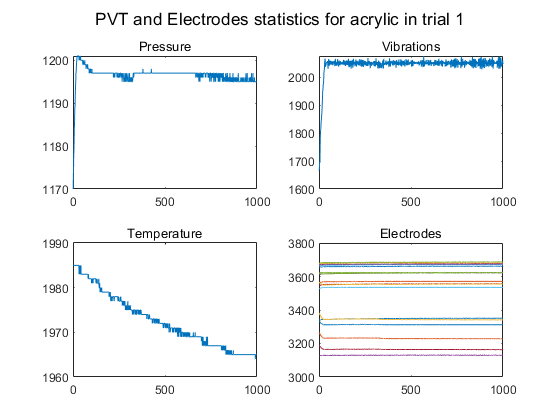
\includegraphics[width=0.47\textwidth]{part1_1}
\end{center}
   \caption{PVT and electrodes statistics for acrylic in trial 1}
\label{fig:1}
\end{figure}

\begin{figure}[h]
\begin{center}
   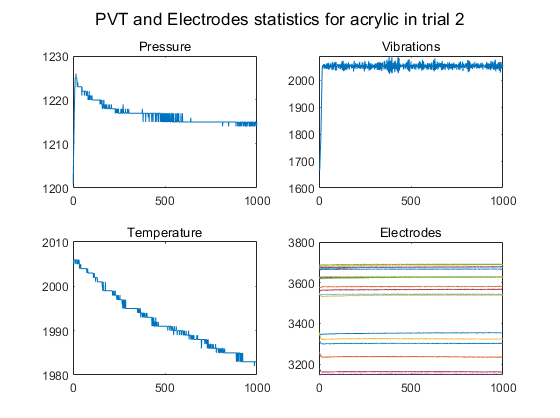
\includegraphics[width=0.47\textwidth]{part1_2}
\end{center}
   \caption{PVT and electrodes statistics for acrylic in trial 2}
\label{fig:2}
\end{figure}

\begin{figure}[h]
\begin{center}
   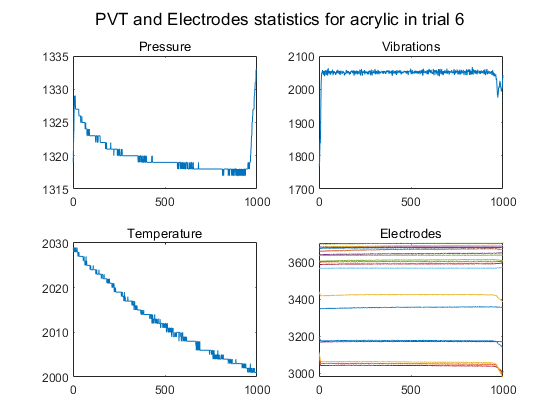
\includegraphics[width=0.47\textwidth]{part1_3}
\end{center}
   \caption{PVT and electrodes statistics for acrylic in trial 6}
\label{fig:3}
\end{figure}

\begin{figure}[h]
\begin{center}
   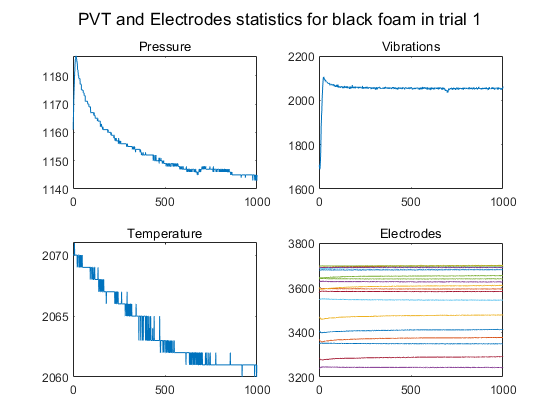
\includegraphics[width=0.47\textwidth]{part1_4}
\end{center}
   \caption{PVT and electrodes statistics for black foam in trial 1}
\label{fig:4}
\end{figure}

\begin{figure}[h]
\begin{center}
   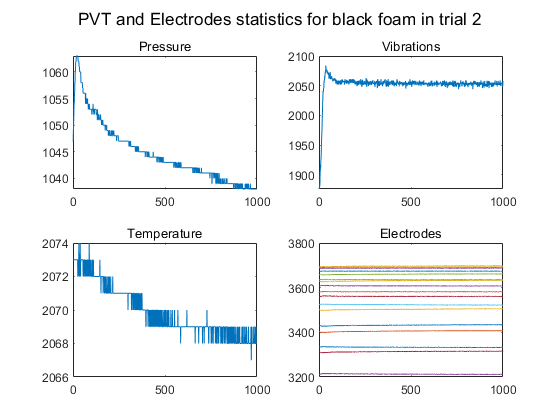
\includegraphics[width=0.47\textwidth]{part1_5}
\end{center}
   \caption{PVT and electrodes statistics for black foam in trial 2}
\label{fig:5}
\end{figure}

\begin{figure}[h]
\begin{center}
   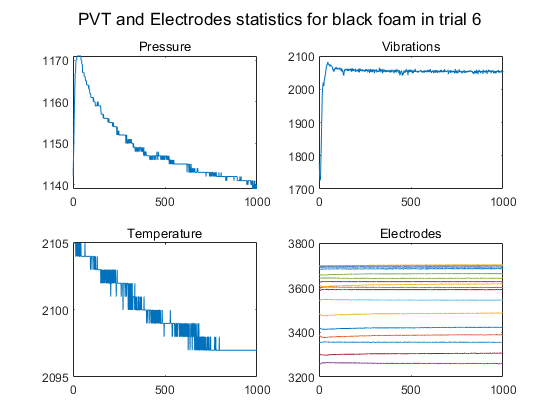
\includegraphics[width=0.47\textwidth]{part1_6}
\end{center}
   \caption{PVT and electrodes statistics for acrylic in trial 6}
\label{fig:6}
\end{figure}

\begin{figure}[h]
\begin{center}
   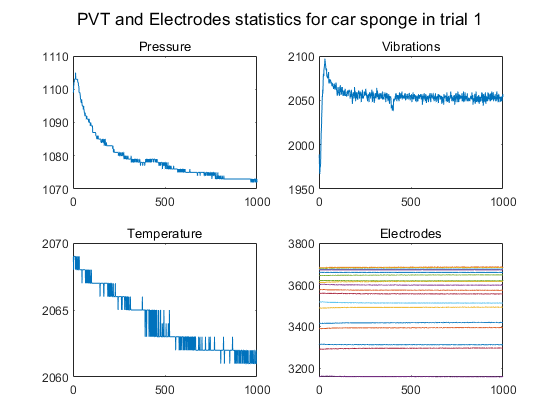
\includegraphics[width=0.47\textwidth]{part1_7}
\end{center}
   \caption{PVT and electrodes statistics for car sponge in trial 1}
\label{fig:7}
\end{figure}

\begin{figure}[h]
\begin{center}
   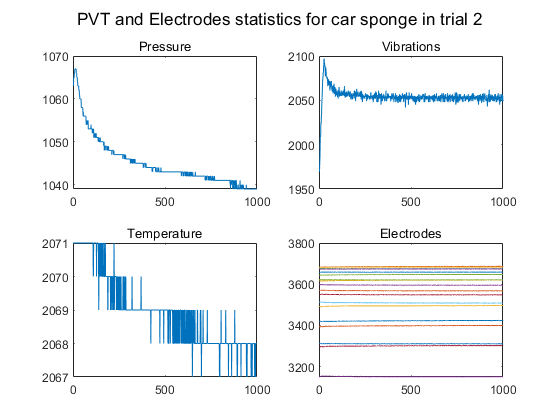
\includegraphics[width=0.47\textwidth]{part1_8}
\end{center}
   \caption{PVT and electrodes statistics for car sponge in trial 2}
\label{fig:8}
\end{figure}

\begin{figure}[h]
\begin{center}
   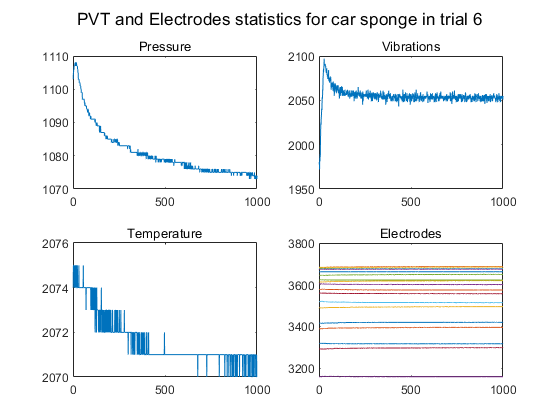
\includegraphics[width=0.47\textwidth]{part1_9}
\end{center}
   \caption{PVT and electrodes statistics for car sponge in trial 6}
\label{fig:9}
\end{figure}

\begin{figure}[h]
\begin{center}
   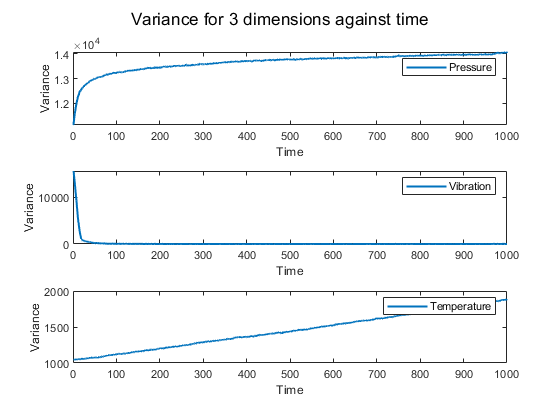
\includegraphics[width=0.47\textwidth]{part1_10}
\end{center}
   \caption{Variance for 3 properties against time}
\label{fig:10}
\end{figure}

\begin{figure}[h]
\begin{center}
   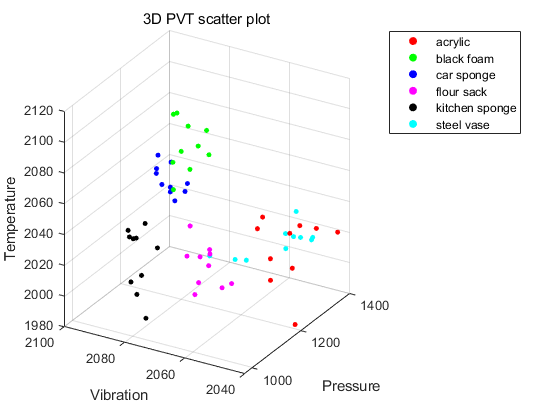
\includegraphics[width=0.47\textwidth]{part3_1}
\end{center}
   \caption{3D PVT}
\label{fig:11}
\end{figure}



\begin{figure}[h]
\begin{center}
   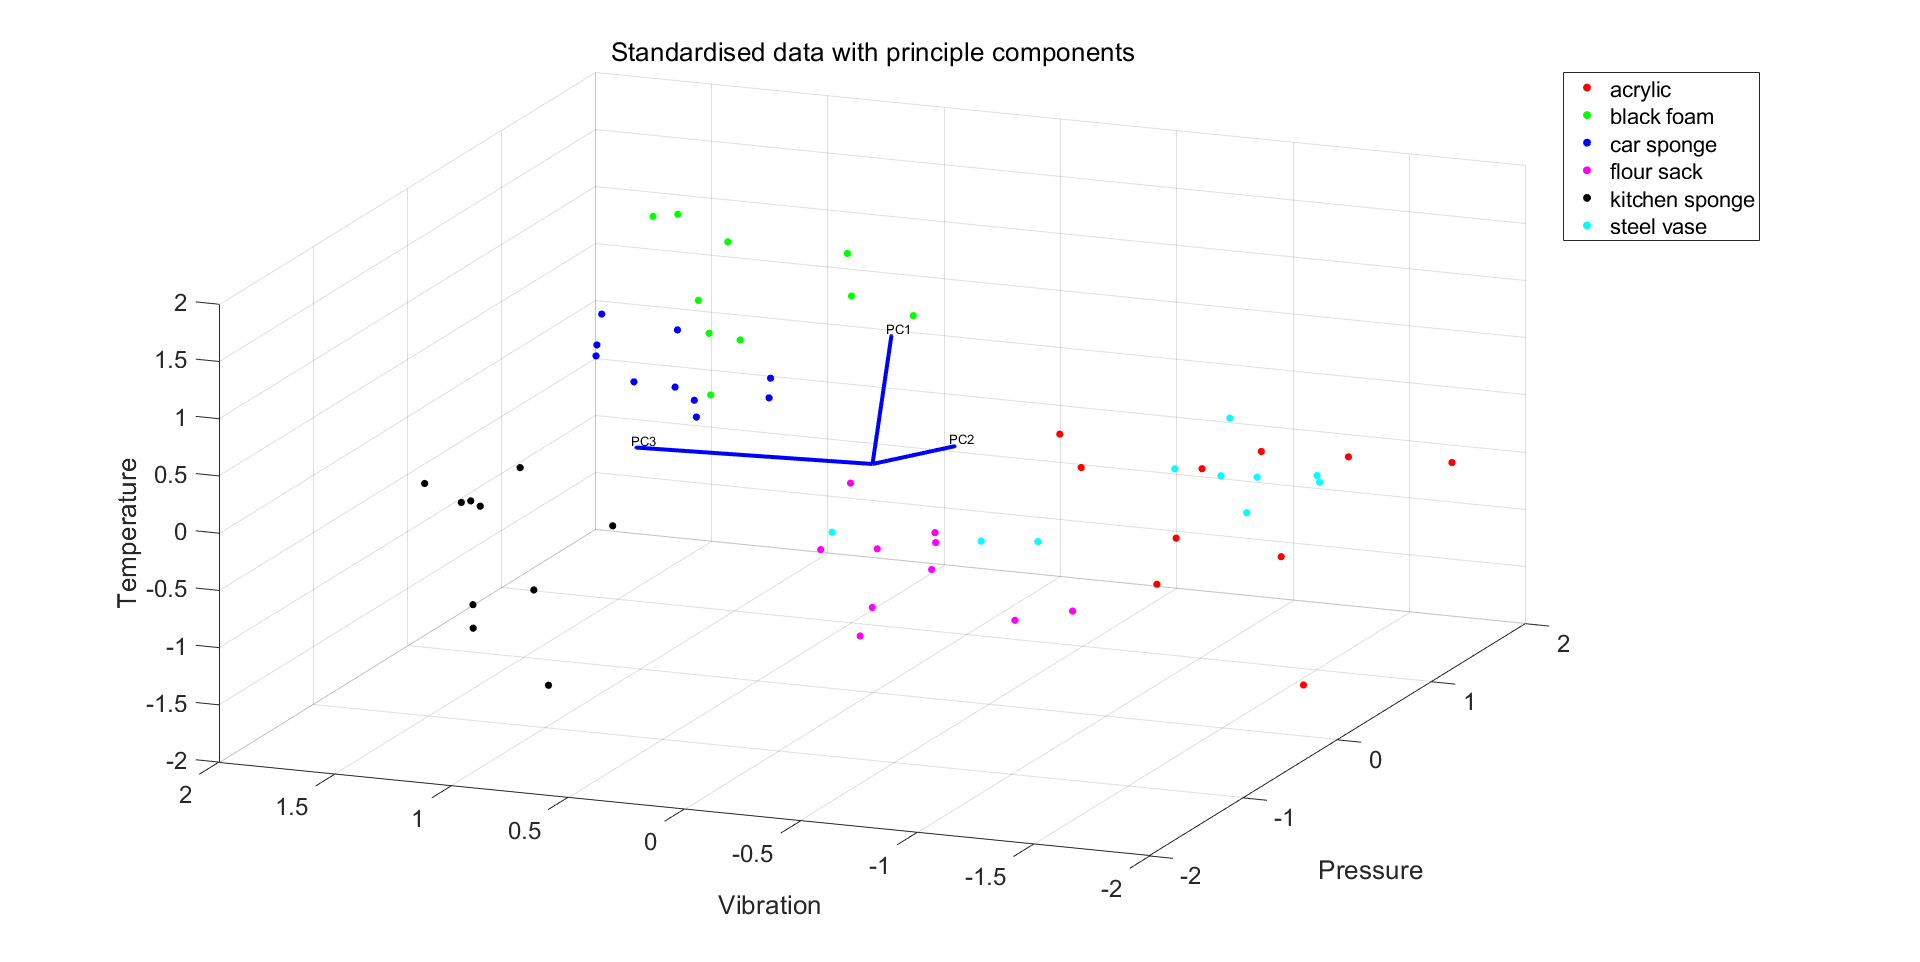
\includegraphics[width=0.47\textwidth]{sec2_part1b}
\end{center}
   \caption{Standardised data}
\label{fig:12}
\end{figure}

\begin{figure}[h]
\begin{center}
   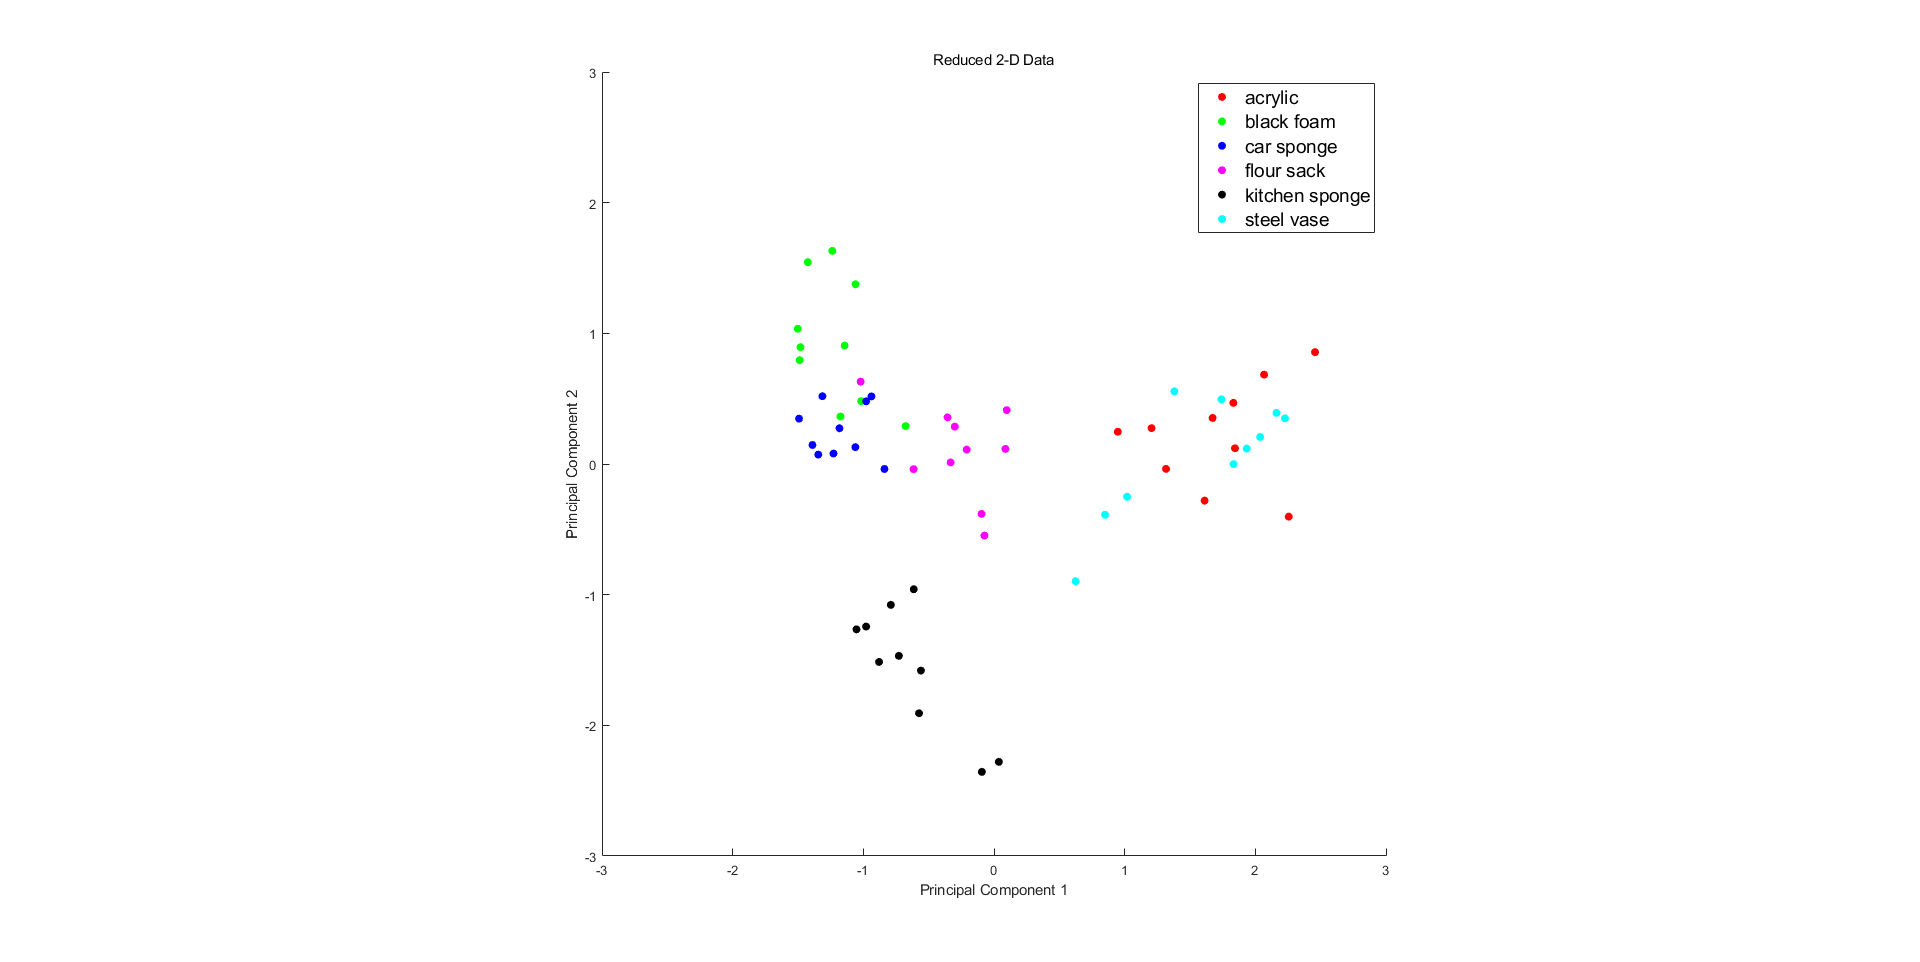
\includegraphics[width=0.47\textwidth]{sec2_part1c}
\end{center}
   \caption{2D data}
\label{fig:13}
\end{figure}

\begin{figure}[h]
\begin{center}
   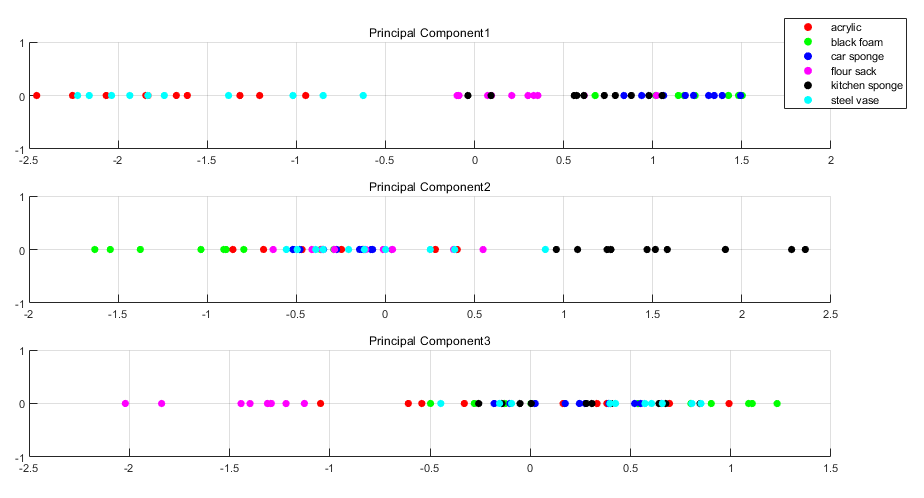
\includegraphics[width=0.47\textwidth]{sec2_part1d}
\end{center}
   \caption{1D data}
\label{fig:14}
\end{figure}

\begin{figure}[h]
\begin{center}
   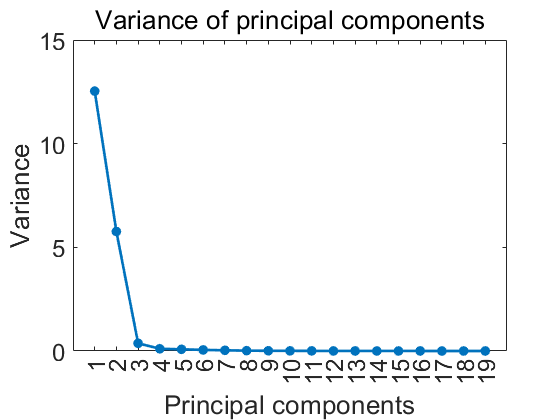
\includegraphics[width=0.47\textwidth]{sec2_part2a}
\end{center}
   \caption{Variance of principle components}
\label{fig:15}
\end{figure}

\begin{figure}[h]
\begin{center}
   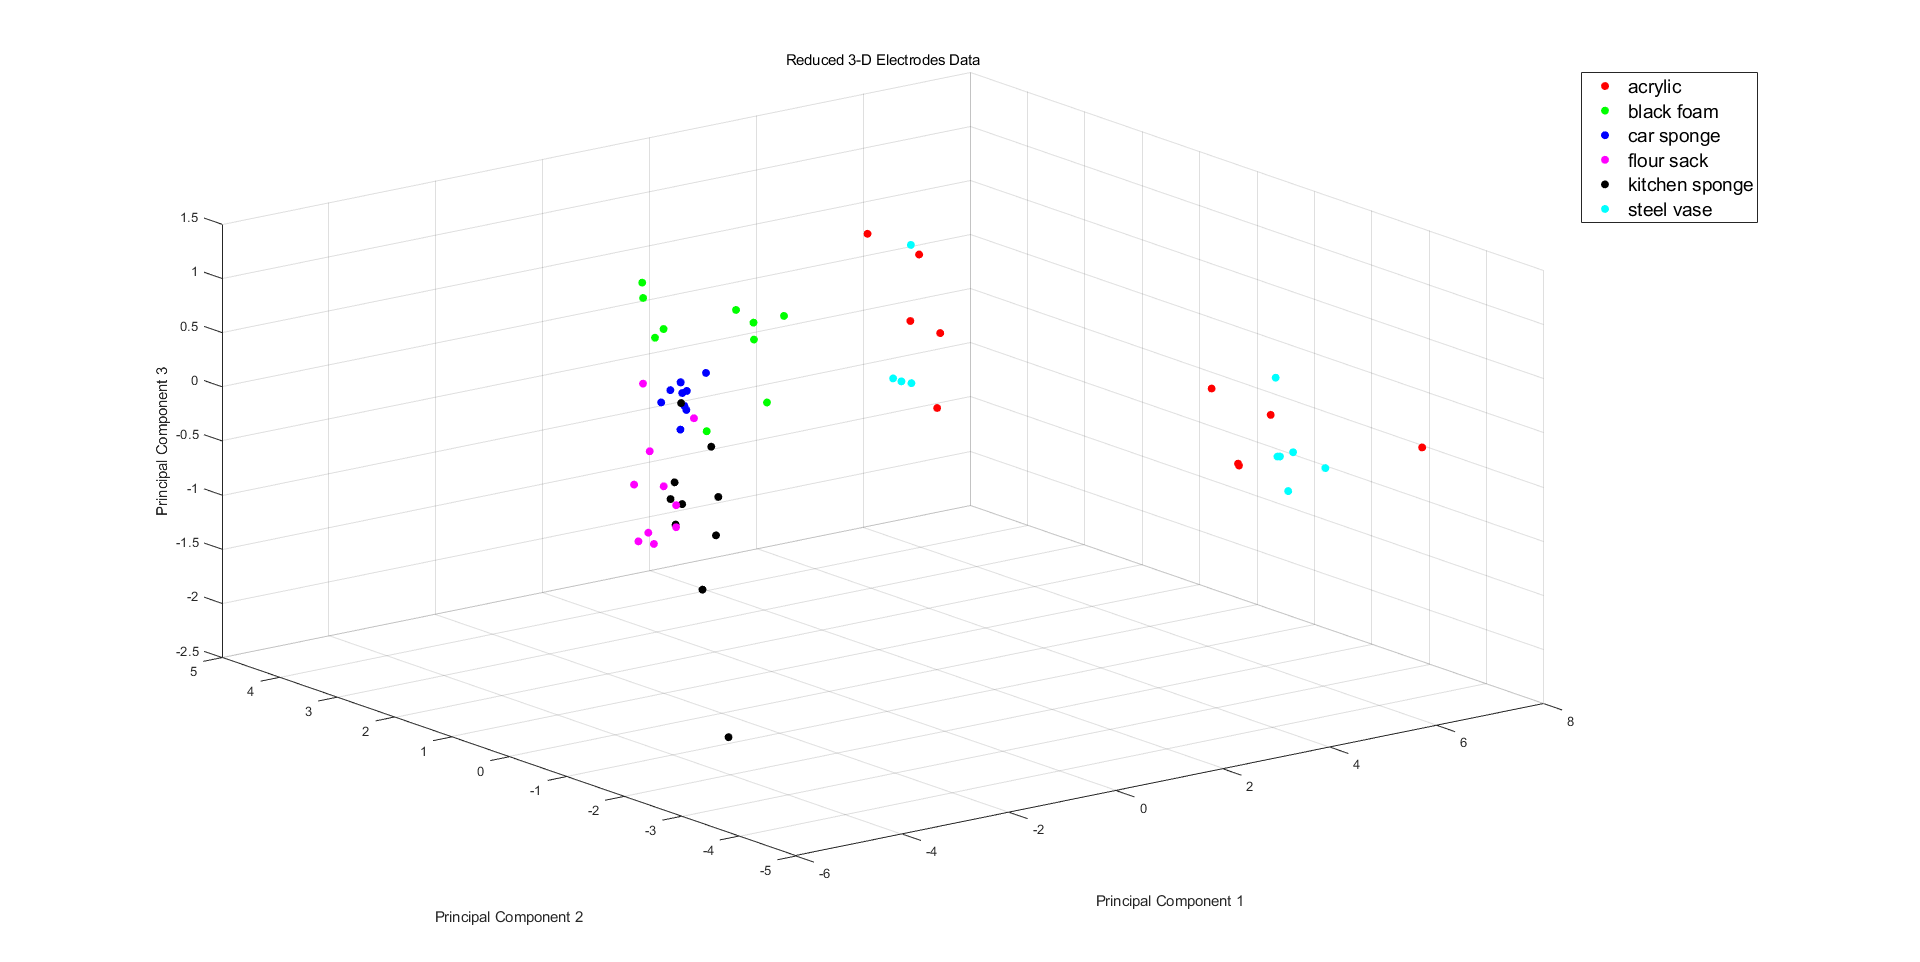
\includegraphics[width=0.47\textwidth]{sec2_part2b}
\end{center}
   \caption{3D electrodes data}
\label{fig:16}
\end{figure}




\begin{figure}[h]
\begin{center}
   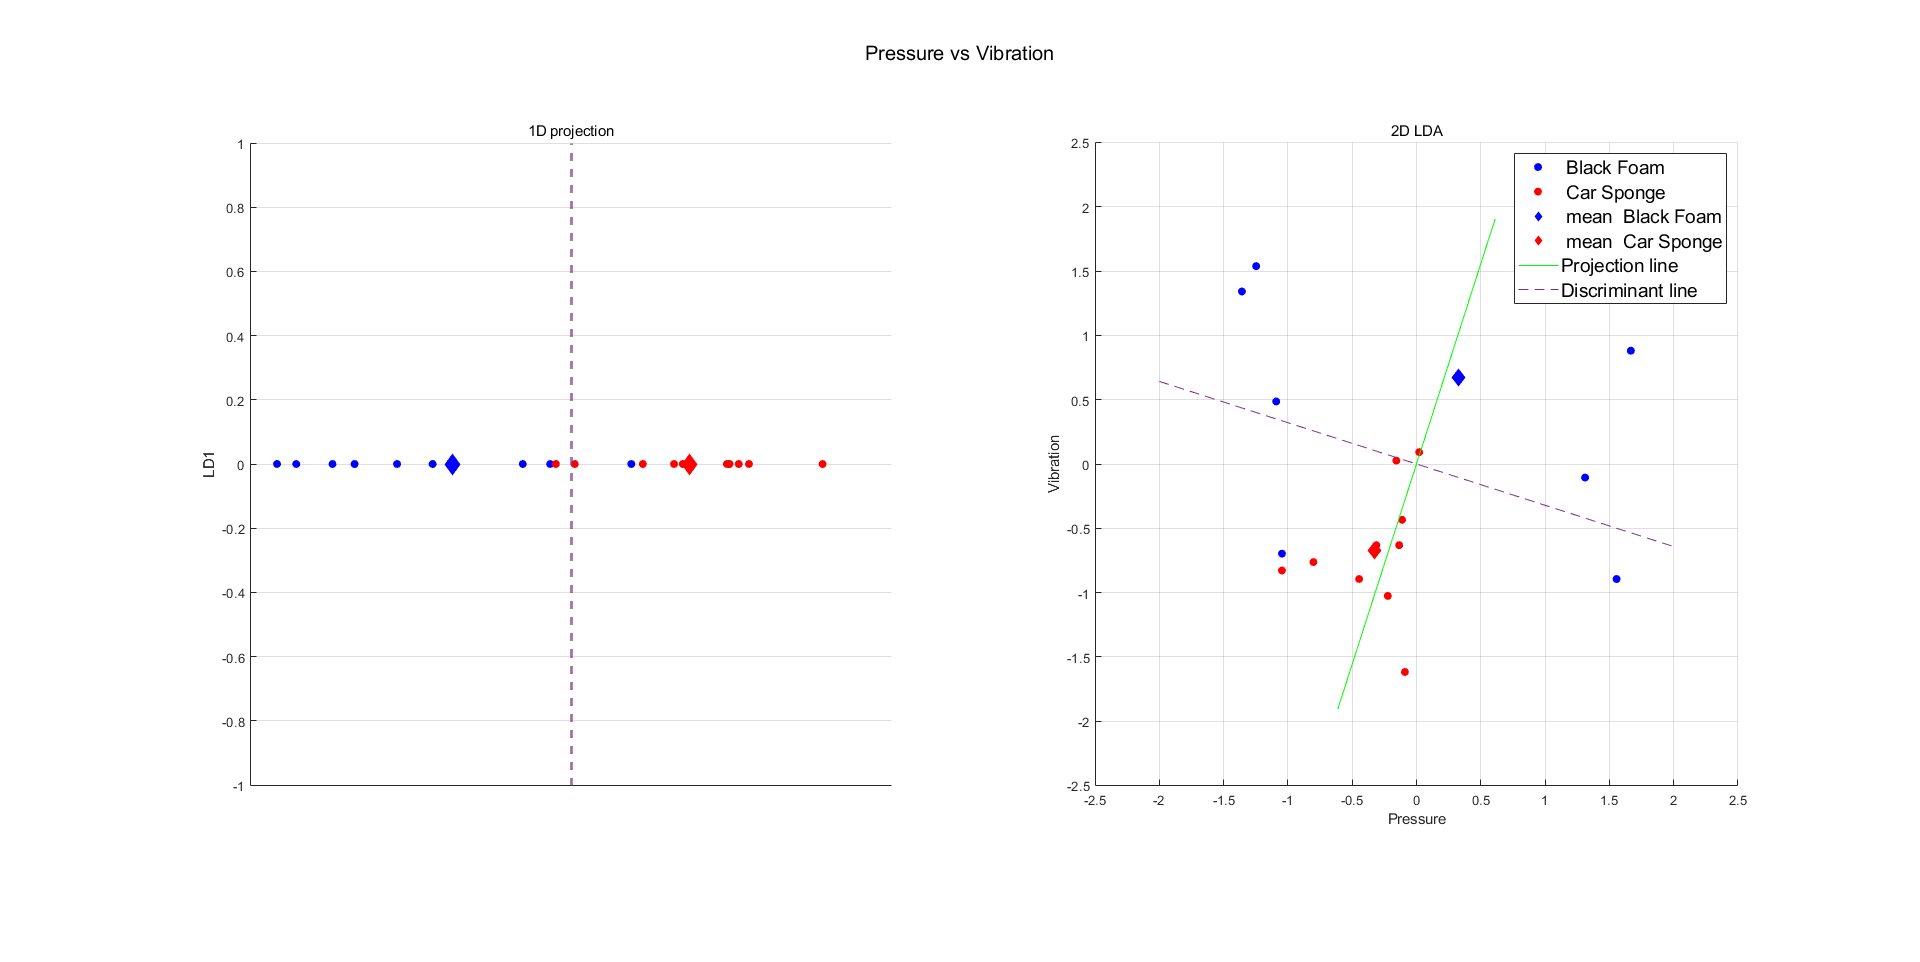
\includegraphics[width=0.47\textwidth]{sec3_part1a_1}
\end{center}
   \caption{Pressure vs Vibration for black foam and car sponge}
\label{fig:17}
\end{figure}

\begin{figure}[h]
\begin{center}
   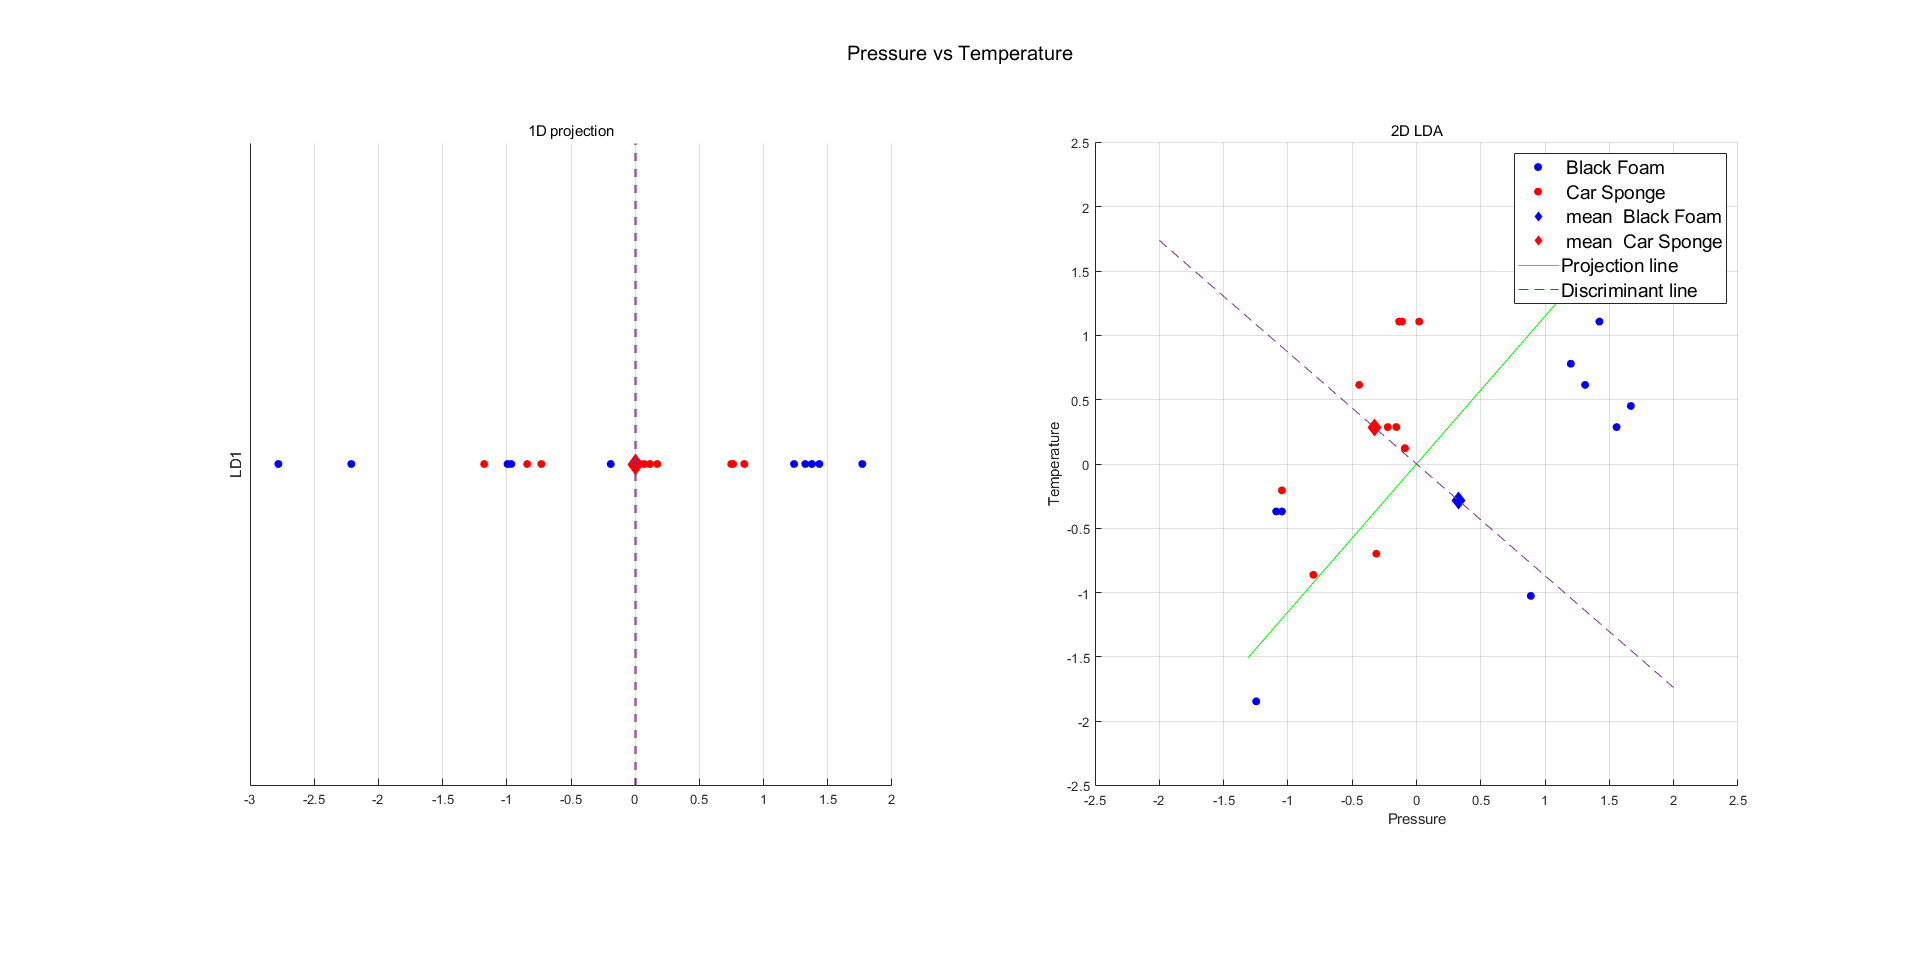
\includegraphics[width=0.47\textwidth]{sec3_part1a_2}
\end{center}
   \caption{Pressure vs Temperature for black foam and car sponge}
\label{fig:18}
\end{figure}

\begin{figure}[h]
\begin{center}
   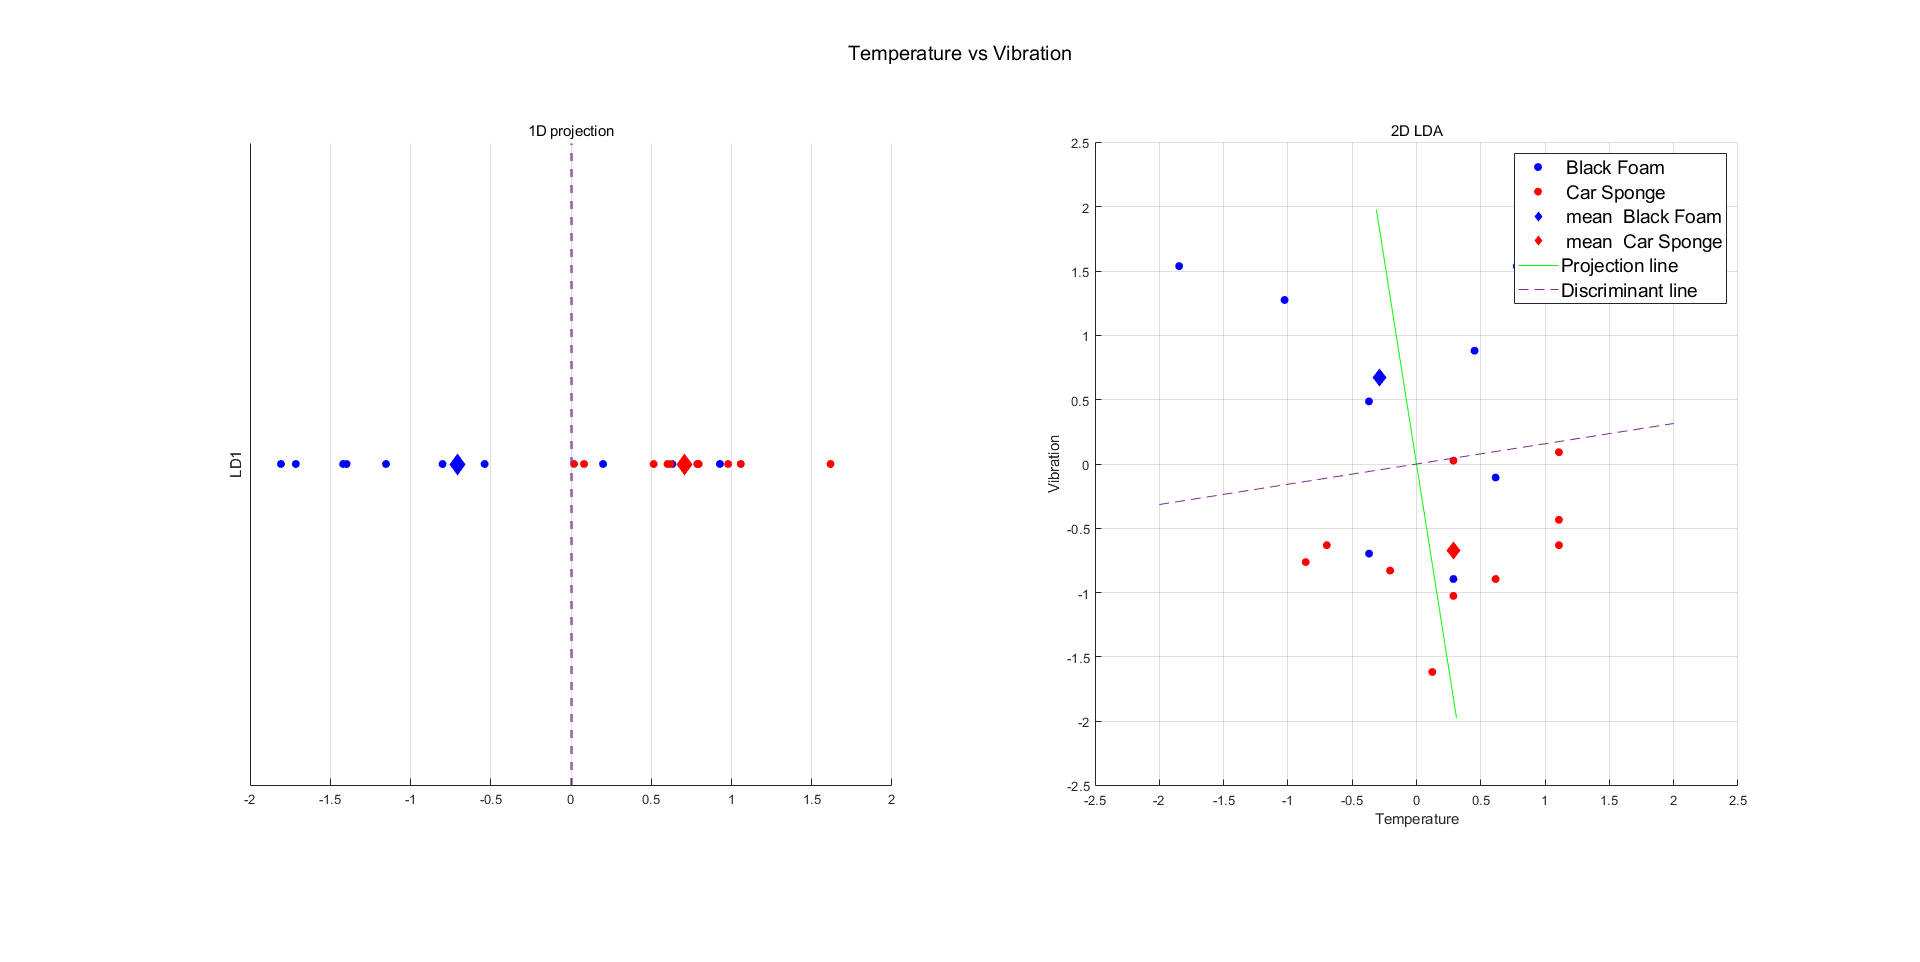
\includegraphics[width=0.47\textwidth]{sec3_part1a_3}
\end{center}
   \caption{Temperature vs Vibration for black foam and car sponge}
\label{fig:19}
\end{figure}

\begin{figure}[h]
\begin{center}
   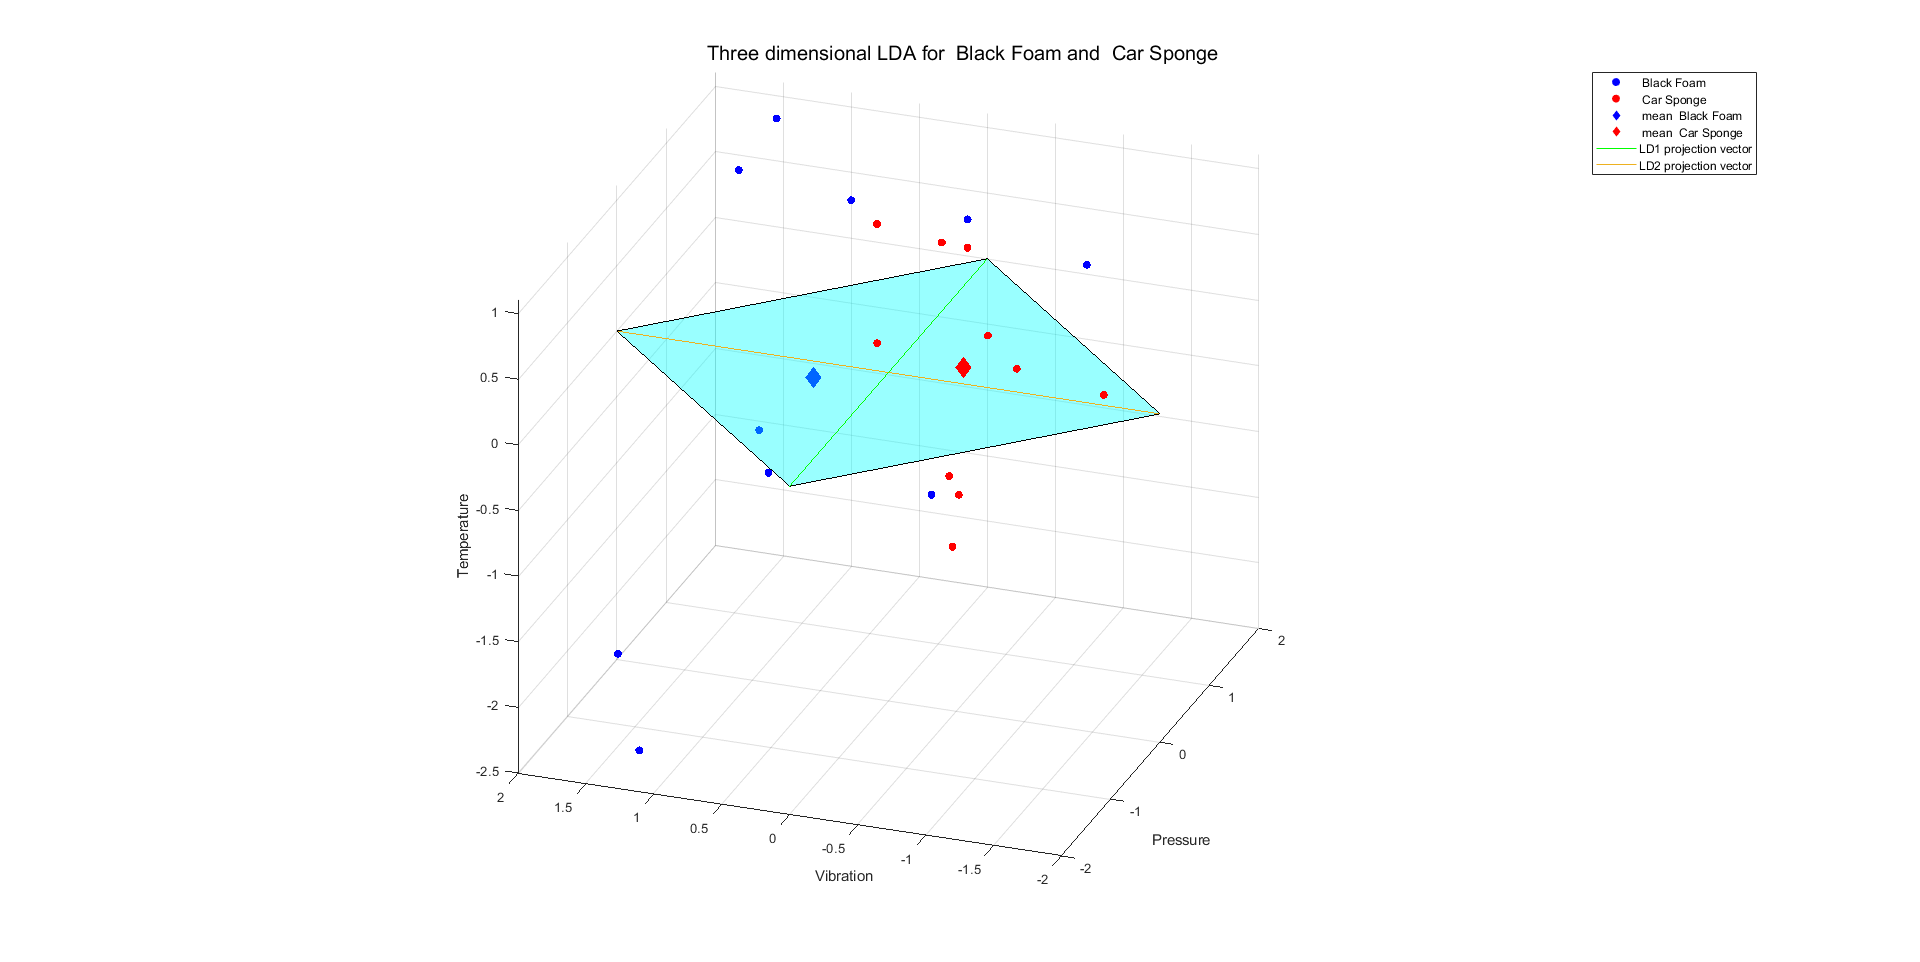
\includegraphics[width=0.47\textwidth]{sec3_part1b_1}
\end{center}
   \caption{3D LDA for black foam and car sponge}
\label{fig:20}
\end{figure}

\begin{figure}[h]
\begin{center}
   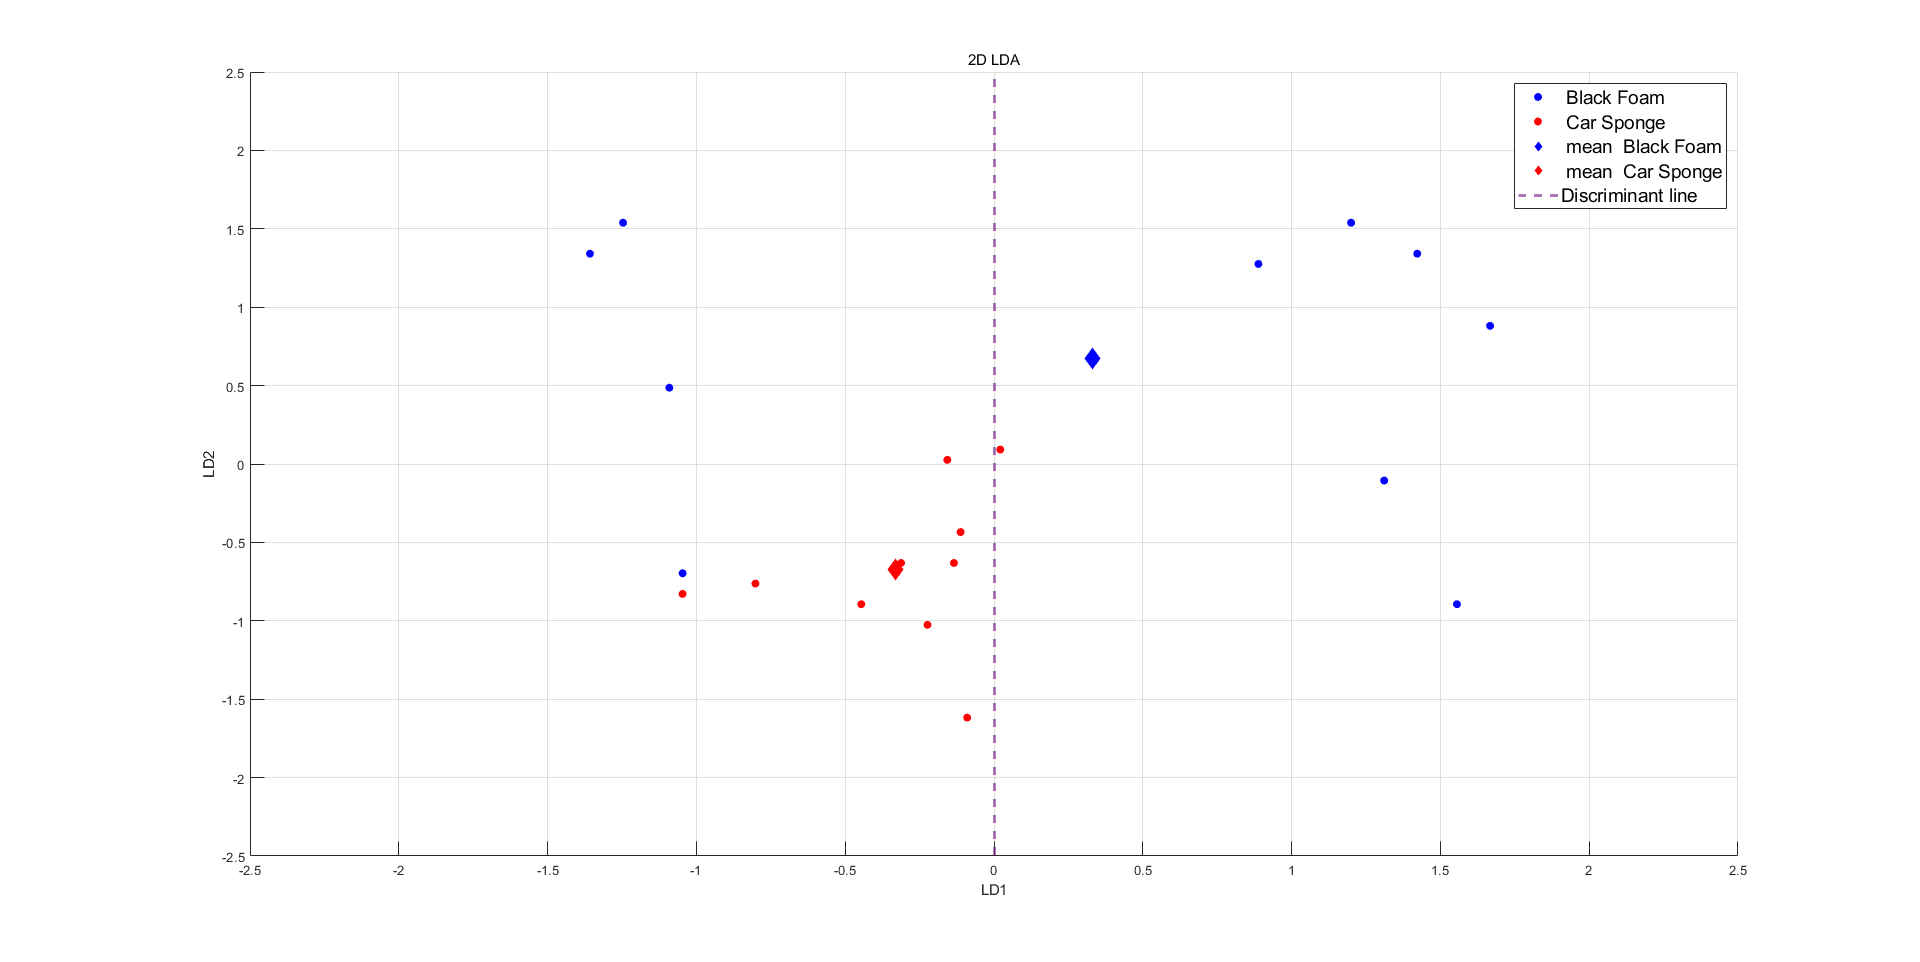
\includegraphics[width=0.47\textwidth]{sec3_part1b_2}
\end{center}
   \caption{2D LDA for black foam and car sponge}
\label{fig:21}
\end{figure}

\begin{figure}[h]
\begin{center}
   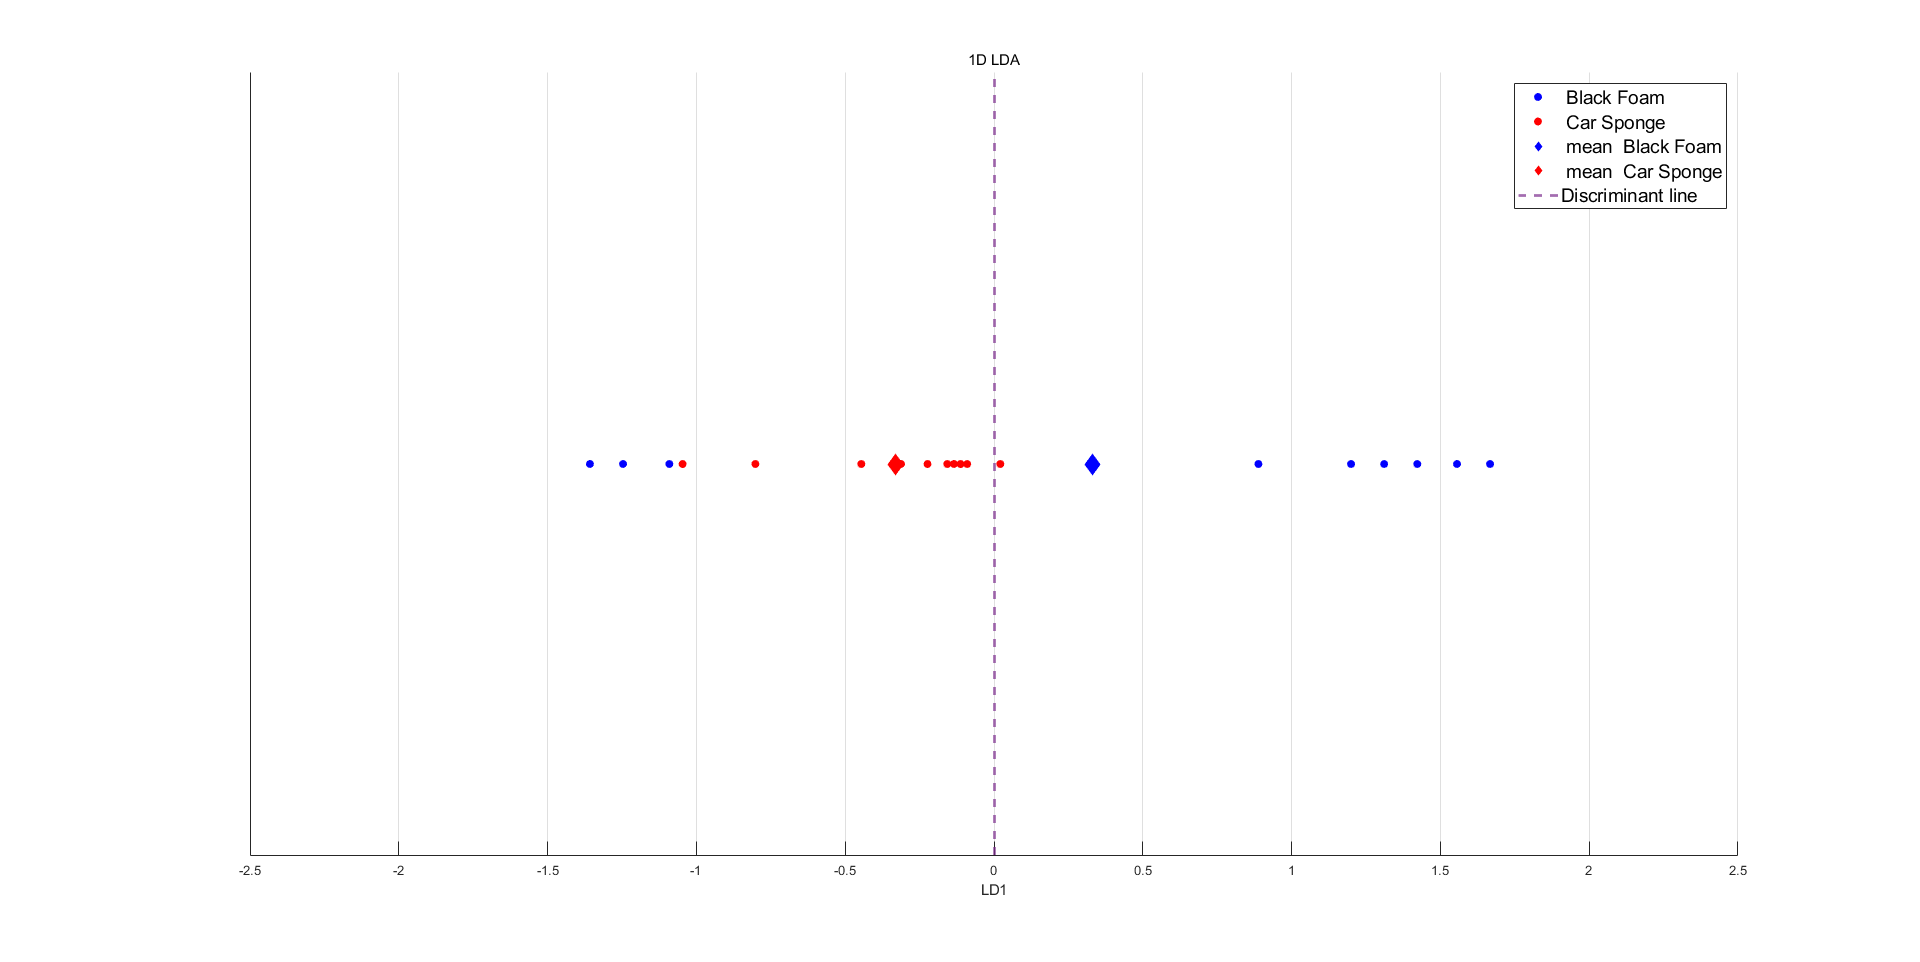
\includegraphics[width=0.47\textwidth]{sec3_part1b_3}
\end{center}
   \caption{1D LDA for black foam and car sponge}
\label{fig:22}
\end{figure}

\begin{figure}[h]
\begin{center}
   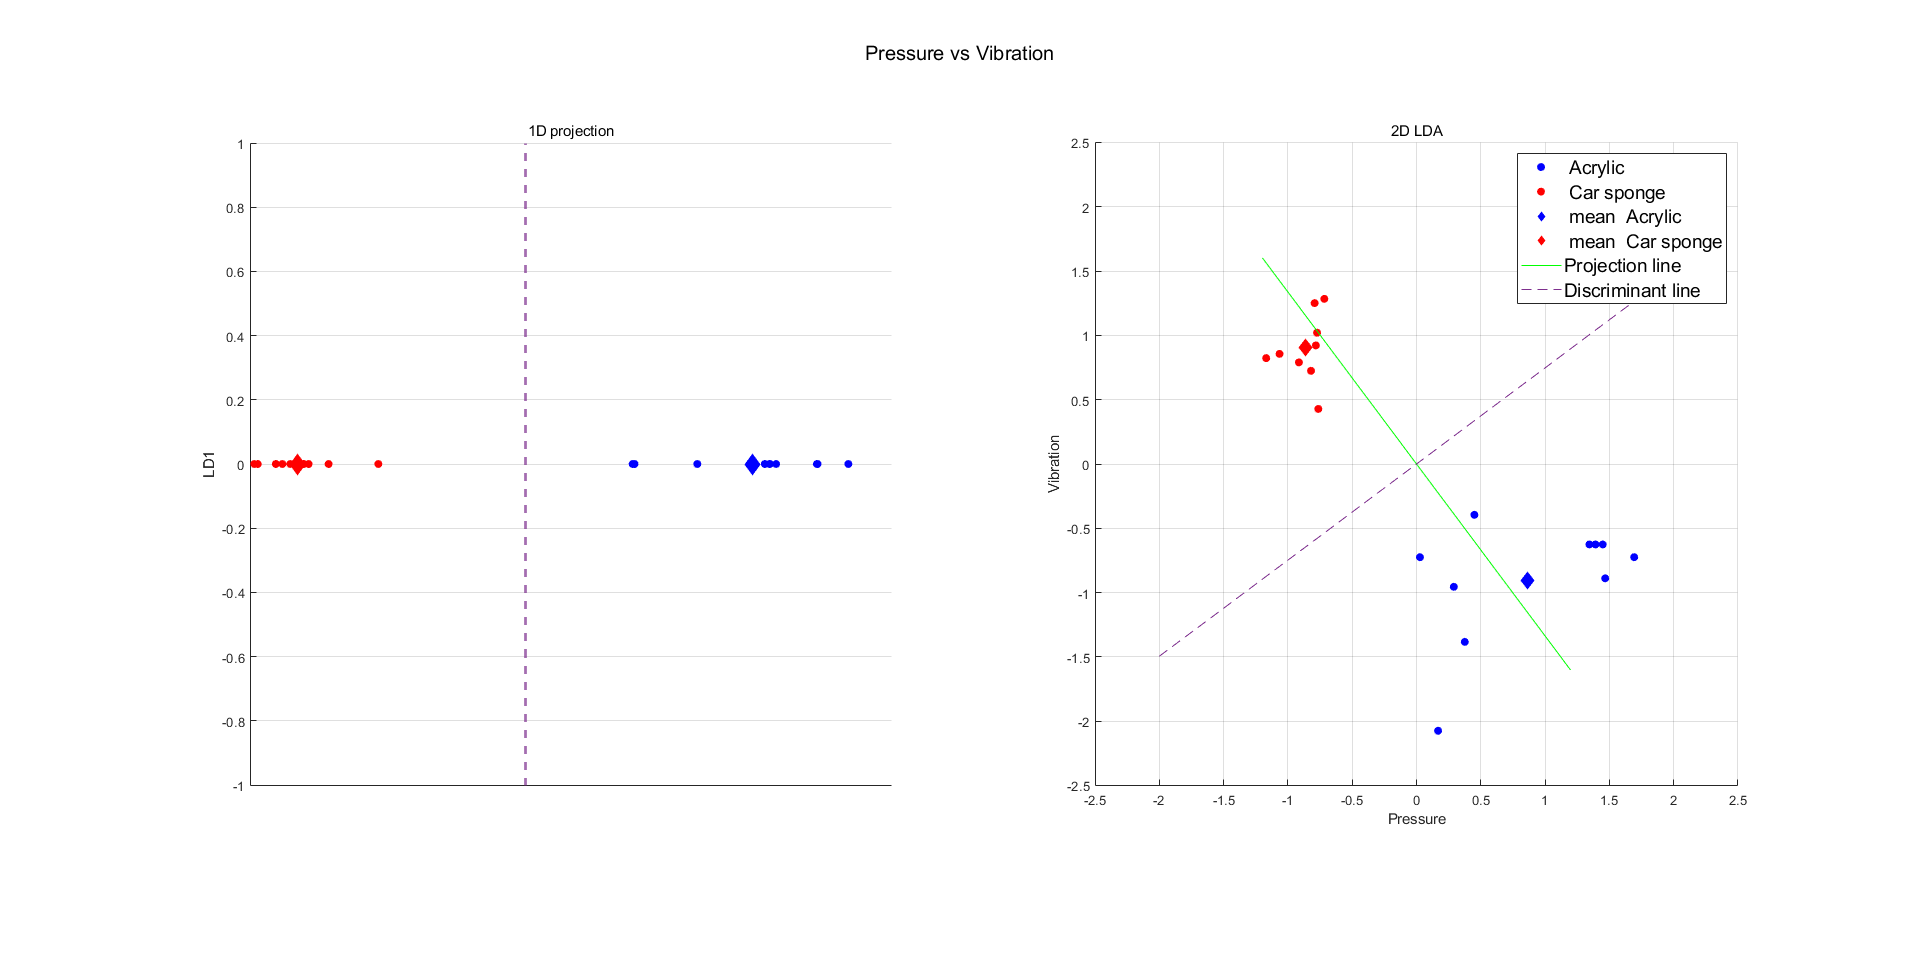
\includegraphics[width=0.47\textwidth]{sec3_part1d_1}
\end{center}
   \caption{Pressure vs Vibration for acrylic and car sponge}
\label{fig:23}
\end{figure}

\begin{figure}[h]
\begin{center}
   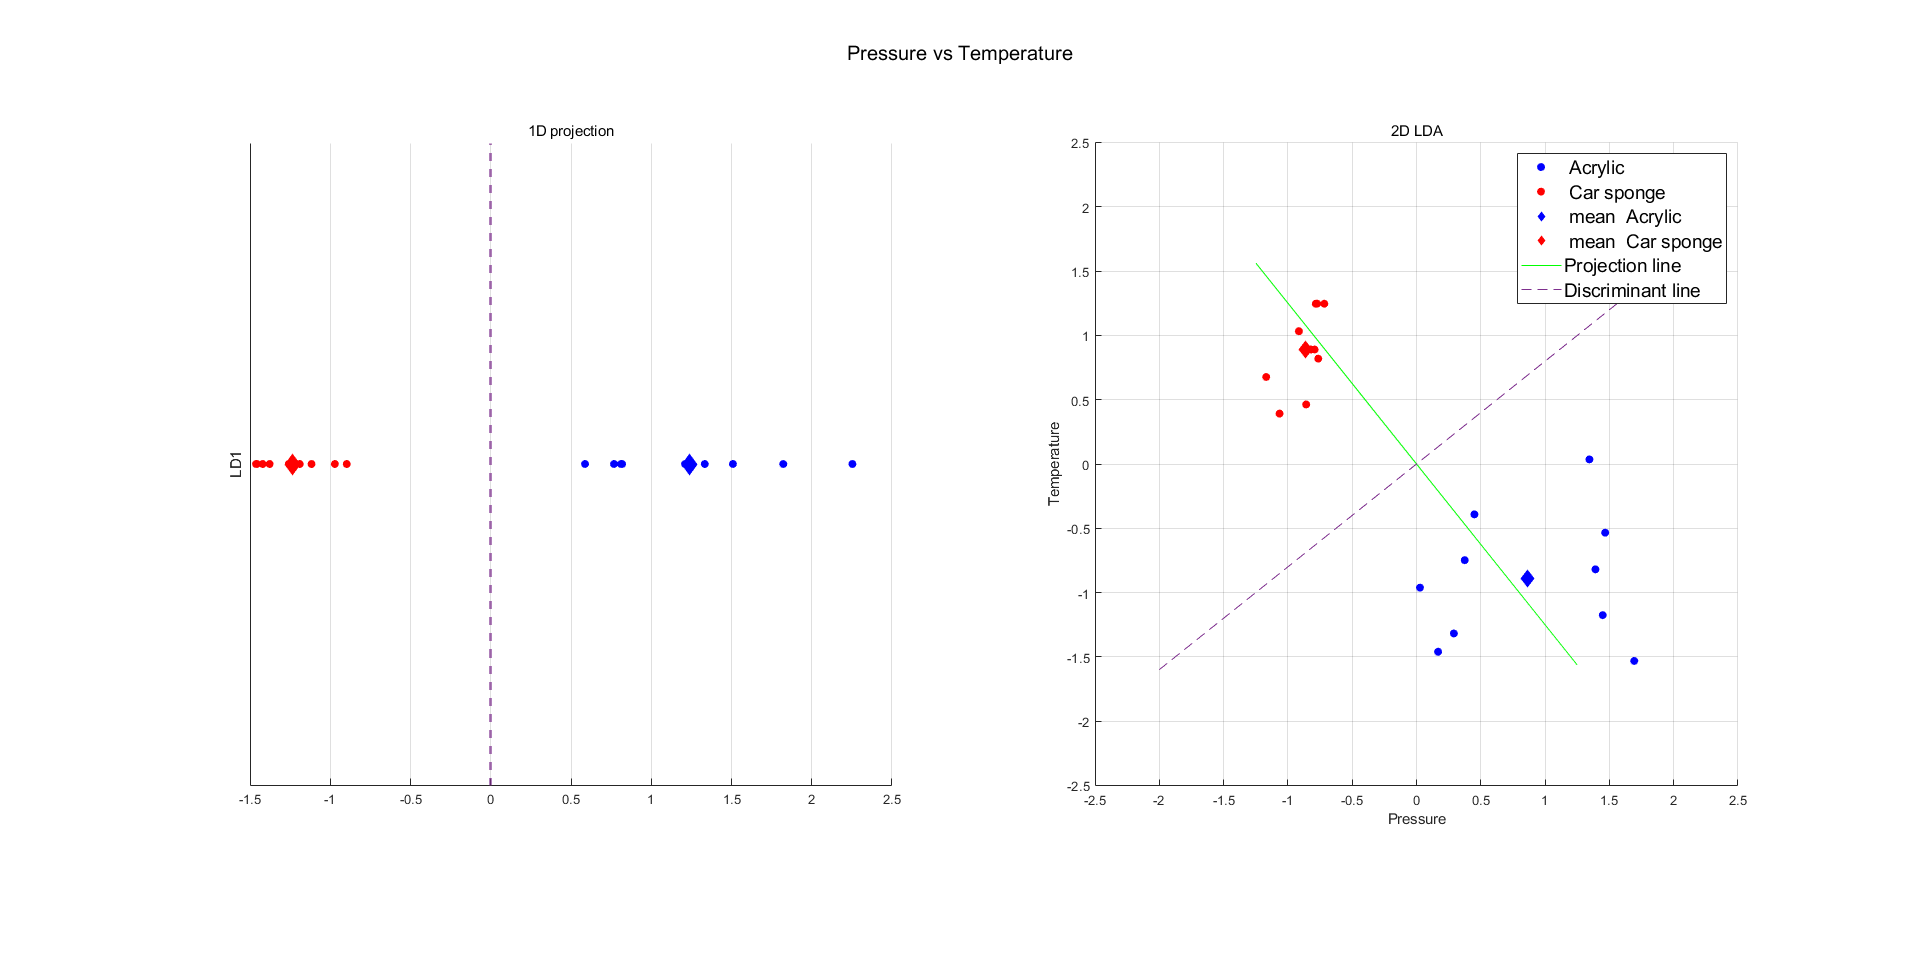
\includegraphics[width=0.47\textwidth]{sec3_part1d_2}
\end{center}
   \caption{Pressure vs Temperature for acrylic and car sponge}
\label{fig:24}
\end{figure}

\begin{figure}[h]
\begin{center}
   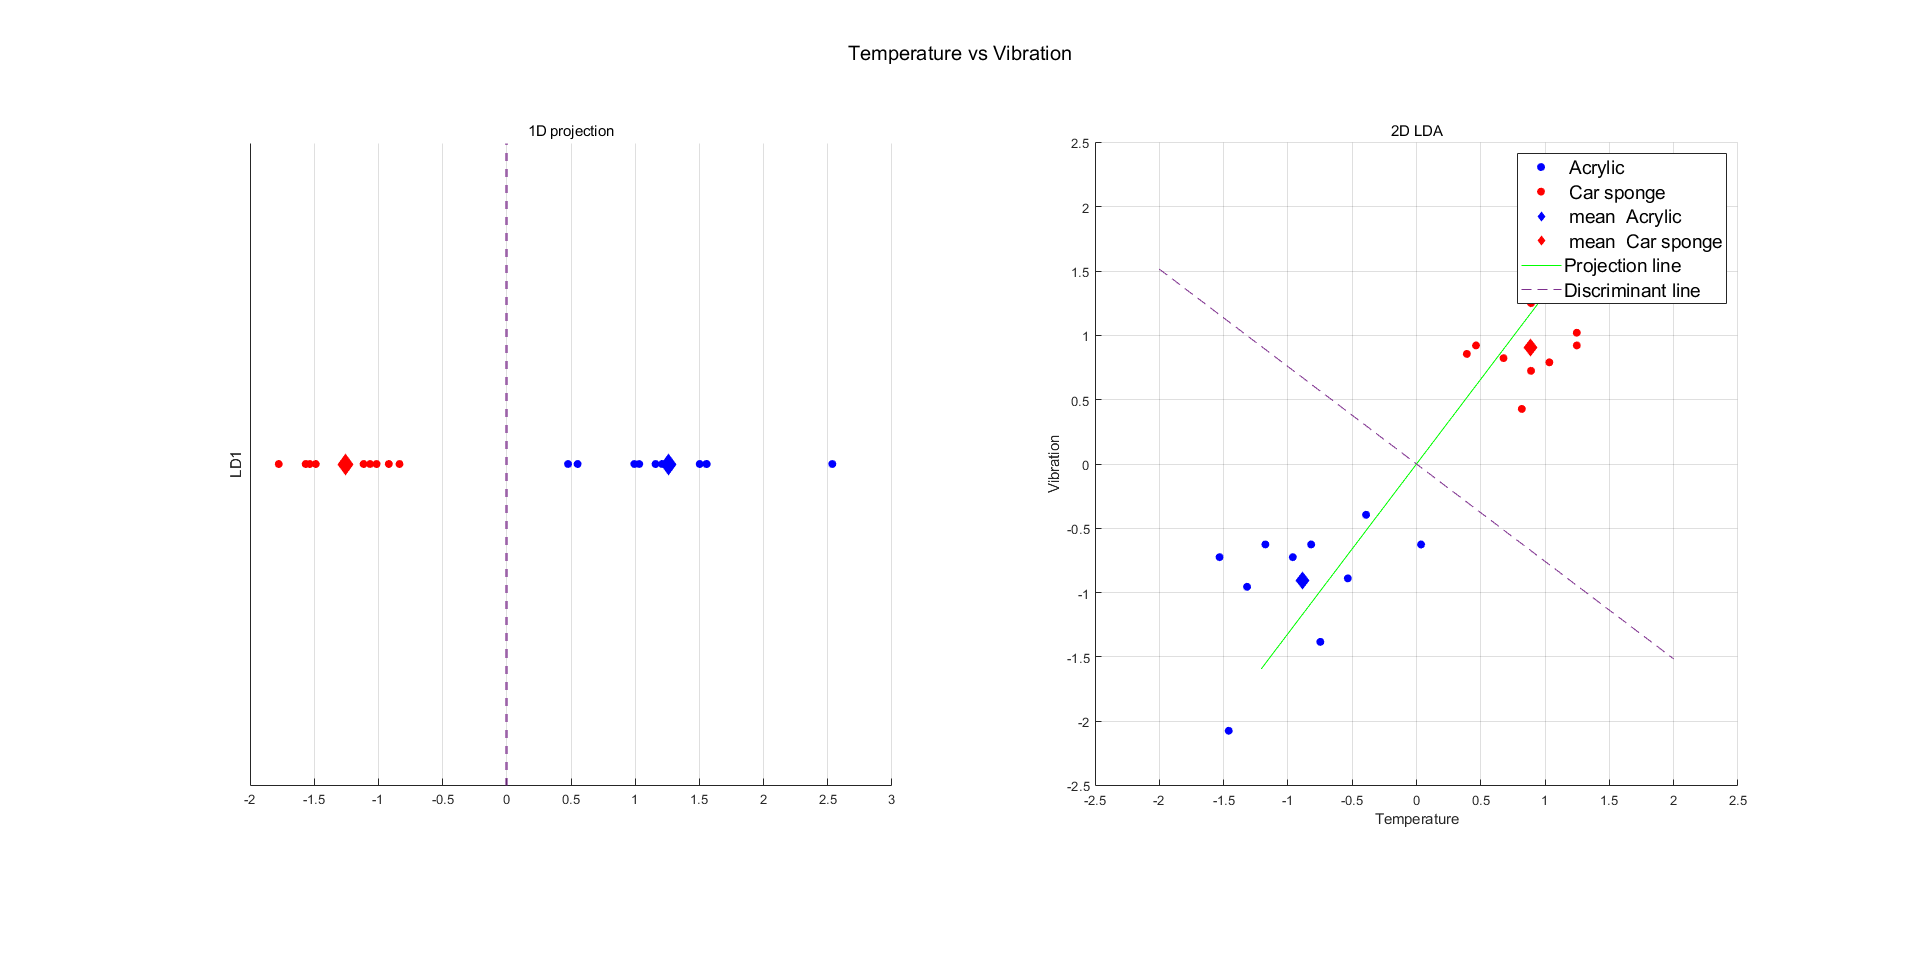
\includegraphics[width=0.47\textwidth]{sec3_part1d_3}
\end{center}
   \caption{Temperature vs Vibration for acrylic and car sponge}
\label{fig:25}
\end{figure}

\begin{figure}[h]
\begin{center}
   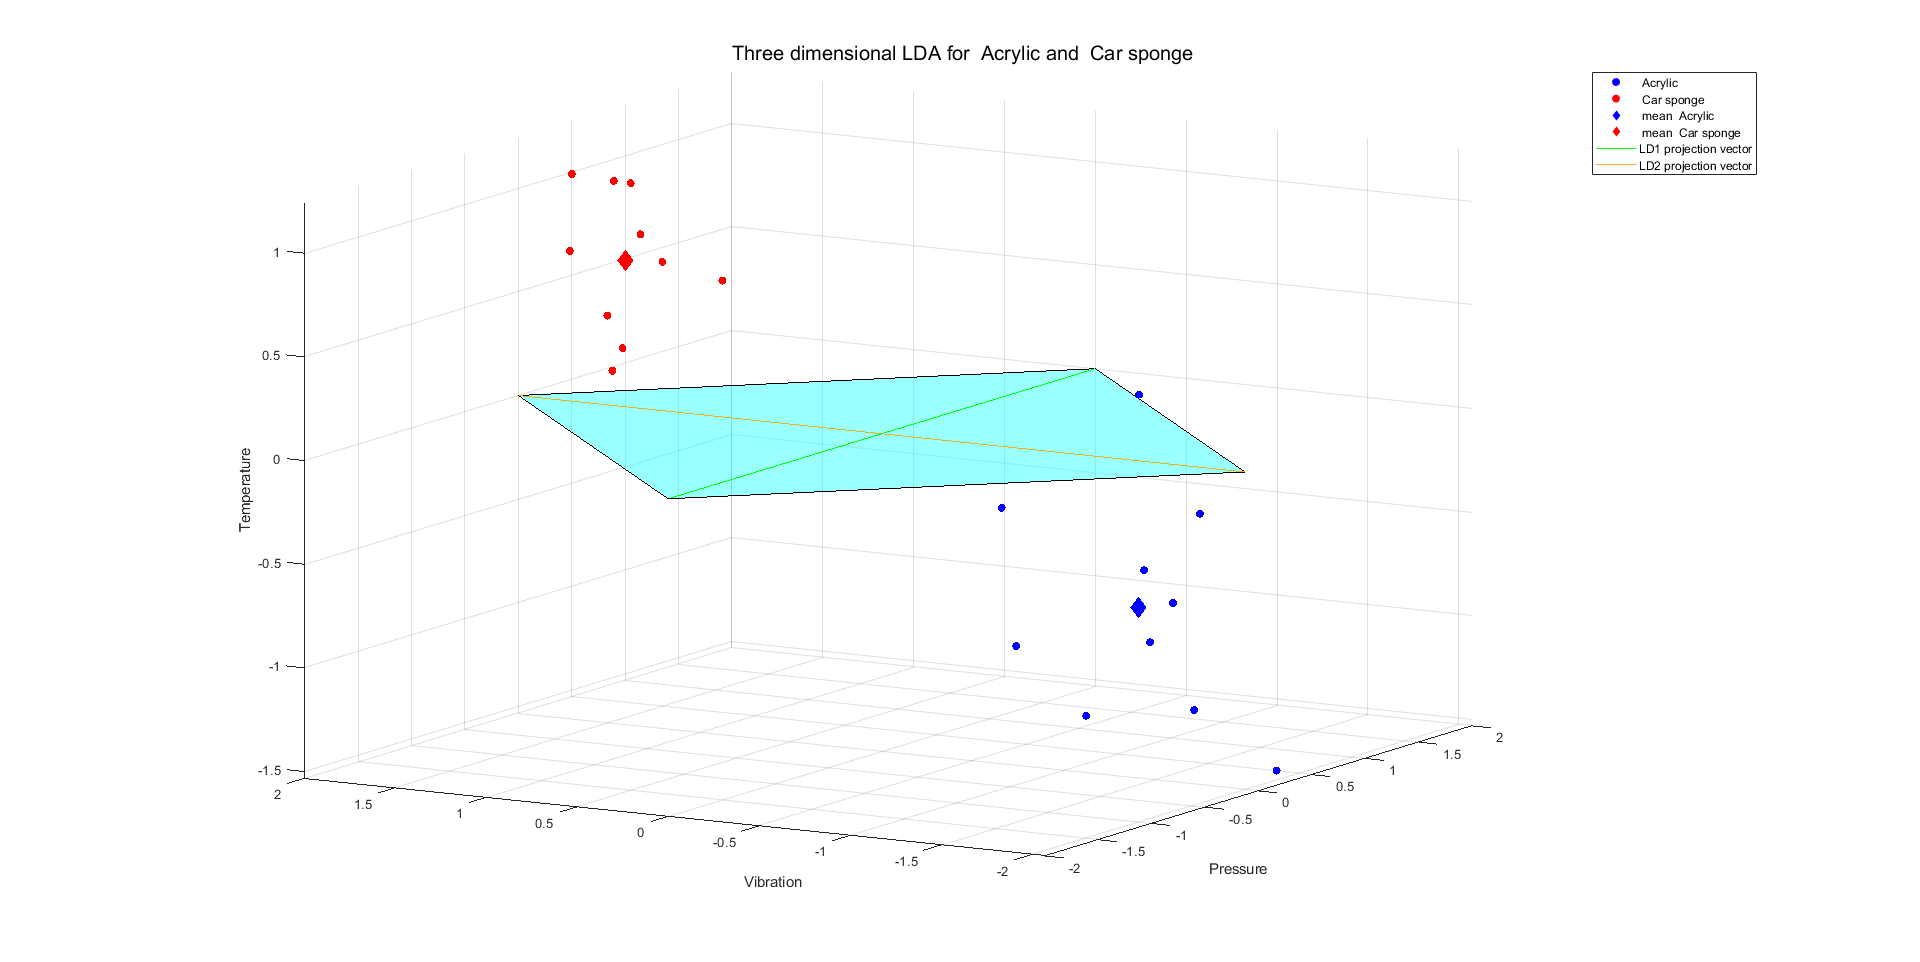
\includegraphics[width=0.47\textwidth]{sec3_part1d_4}
\end{center}
   \caption{3D LDA for acrylic and car sponge}
\label{fig:26}
\end{figure}

\begin{figure}[h]
\begin{center}
   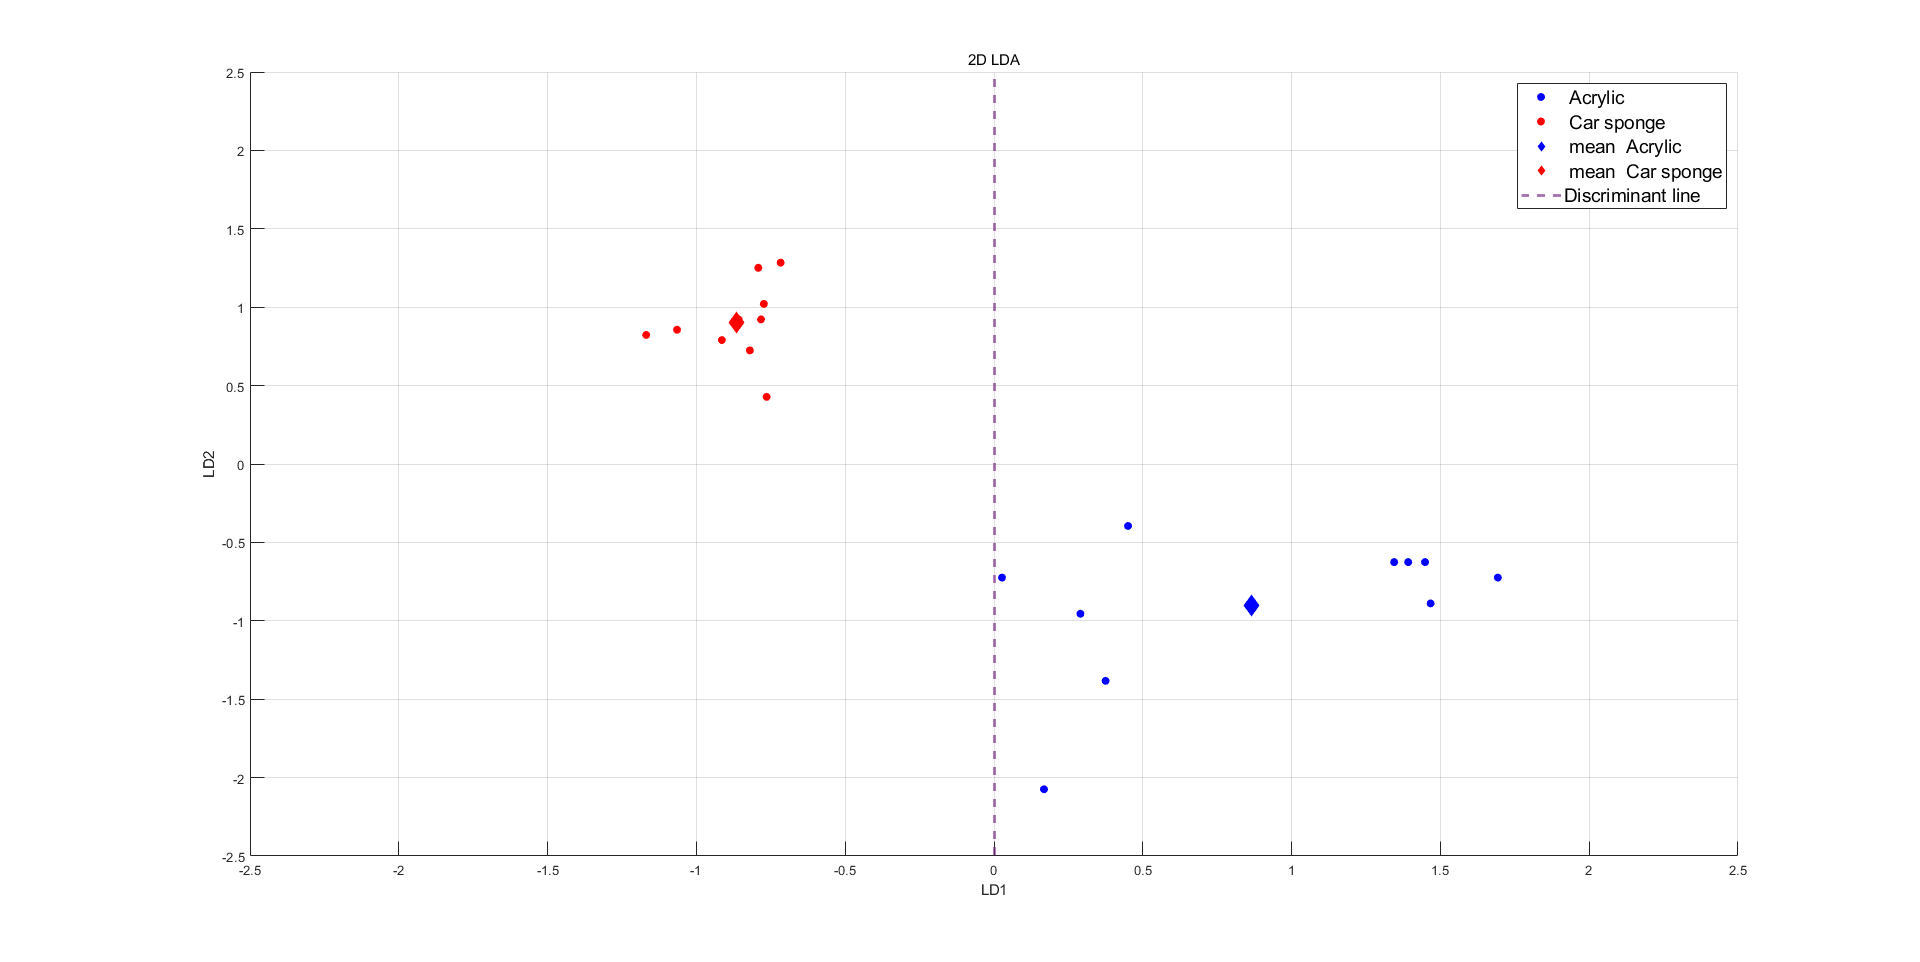
\includegraphics[width=0.47\textwidth]{sec3_part1d_5}
\end{center}
   \caption{2D LDA for acrylic and car sponge}
\label{fig:27}
\end{figure}

\begin{figure}[h]
\begin{center}
   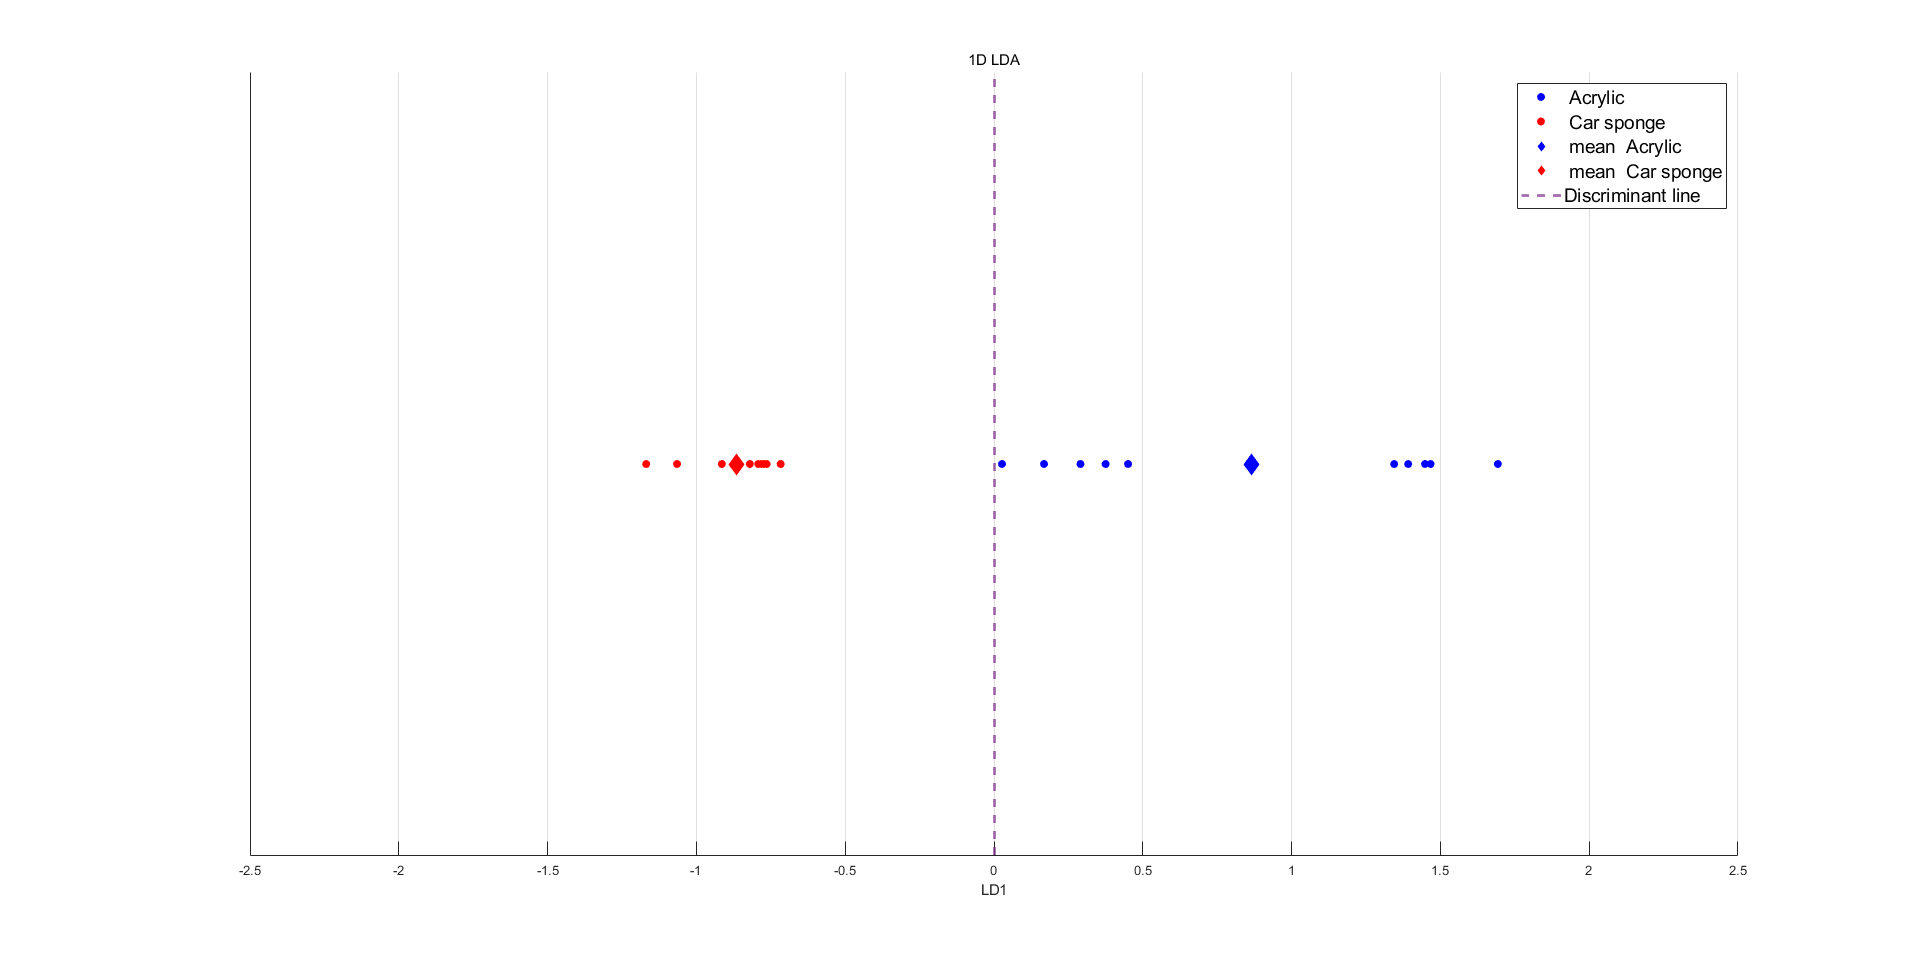
\includegraphics[width=0.47\textwidth]{sec3_part1d_6}
\end{center}
   \caption{1D LDA for acrylic and car sponge}
\label{fig:28}
\end{figure}


\begin{figure}[h]
\begin{center}
   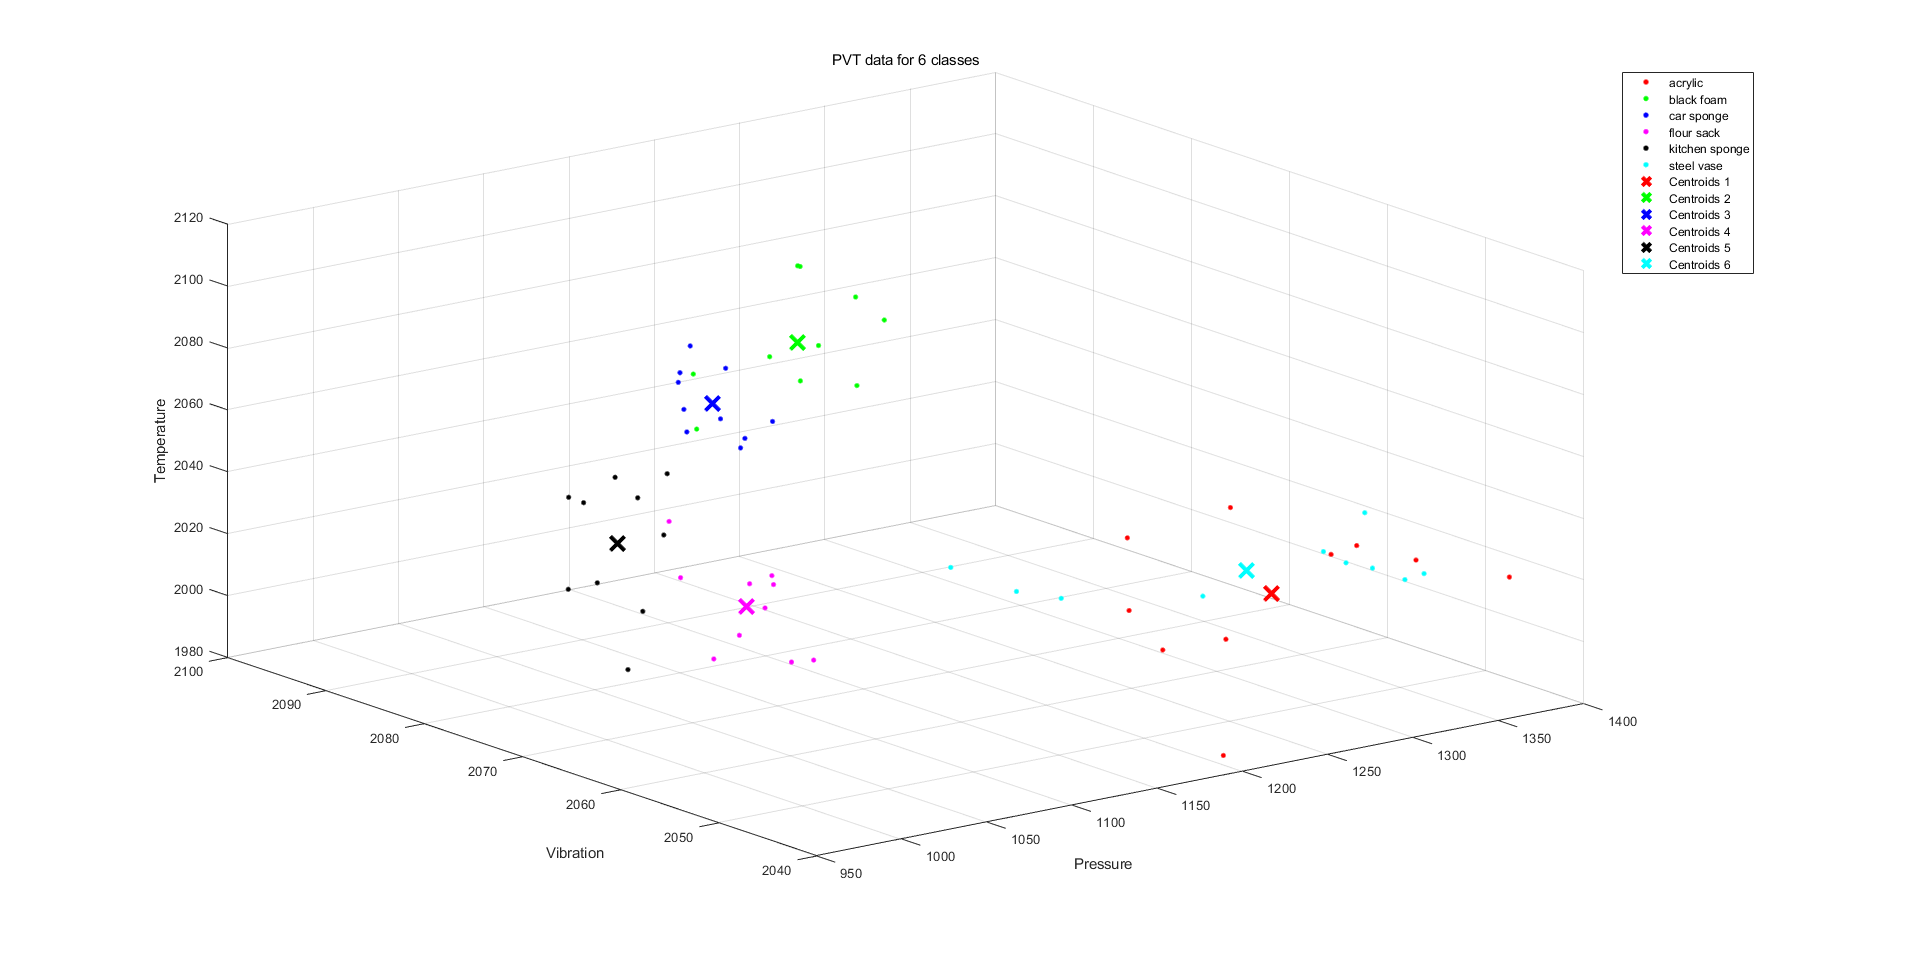
\includegraphics[width=0.47\textwidth]{sec4_part1a_1}
\end{center}
   \caption{Original data classification}
\label{fig:29}
\end{figure}

\begin{figure}[h]
\begin{center}
   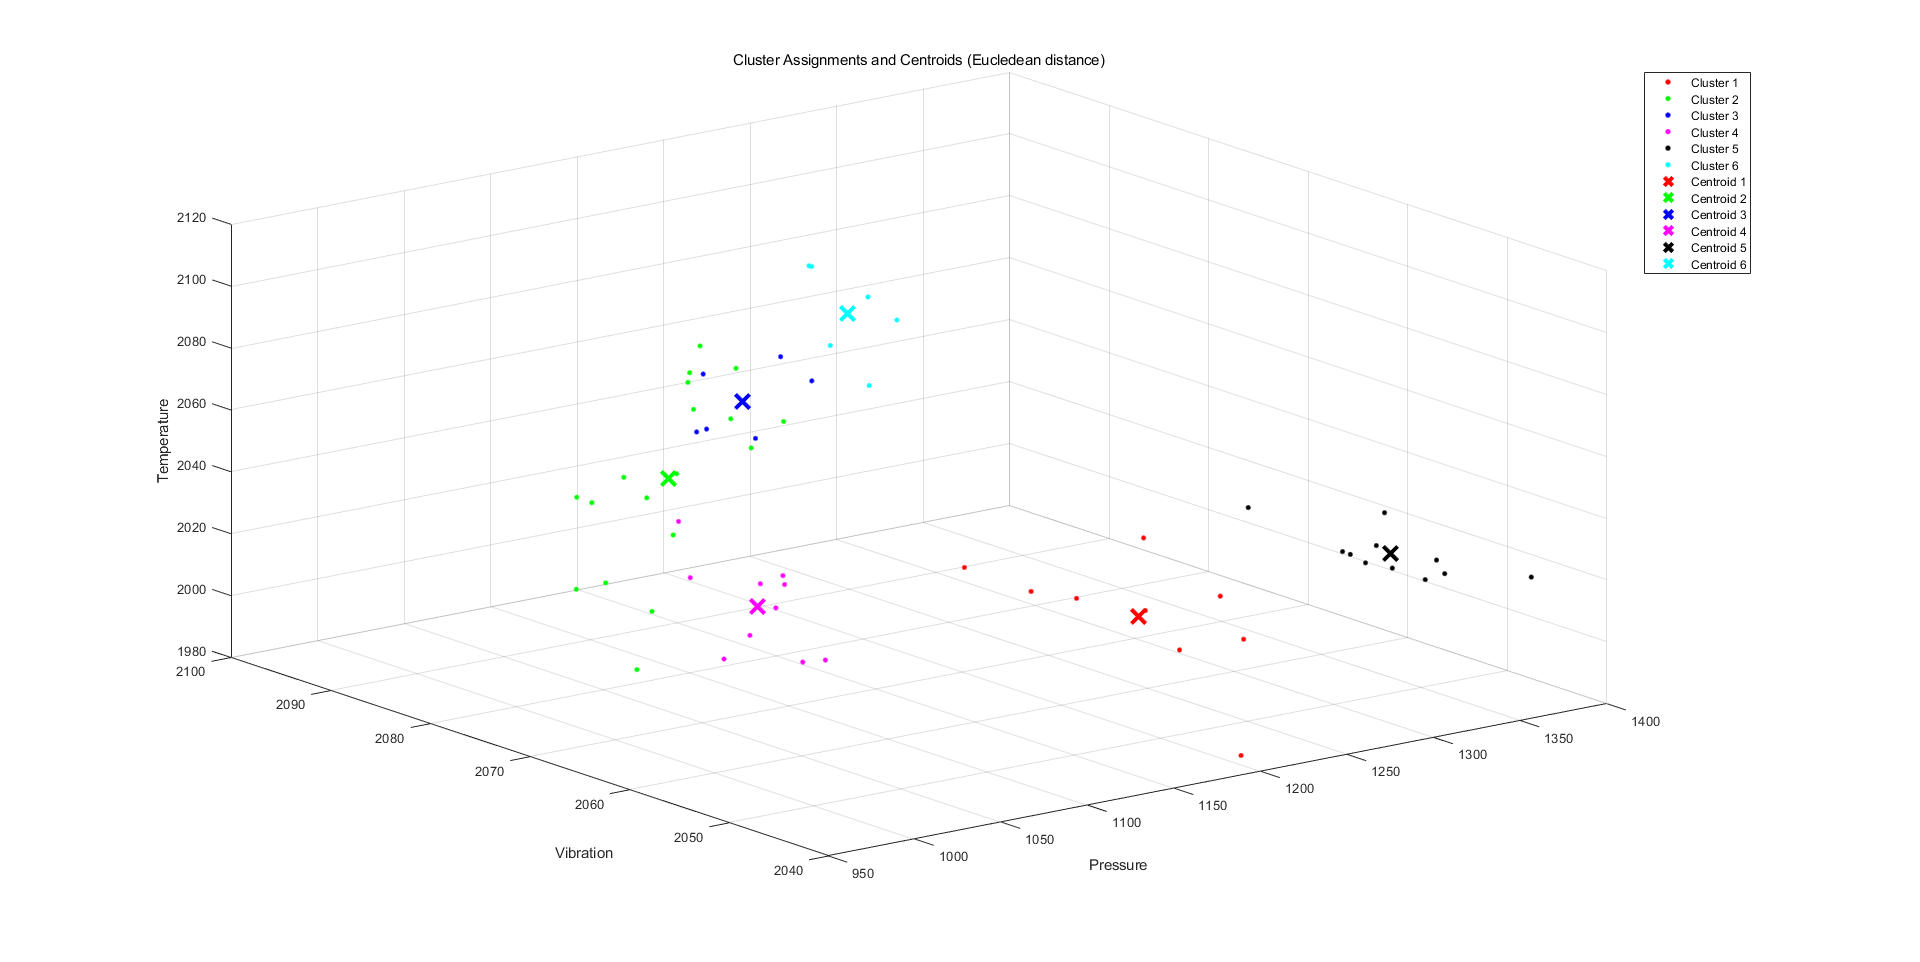
\includegraphics[width=0.47\textwidth]{sec4_part1a_2}
\end{center}
   \caption{K-means cluster algorithm with Eucledean distance}
\label{fig:30}
\end{figure}

\begin{figure}[h]
\begin{center}
   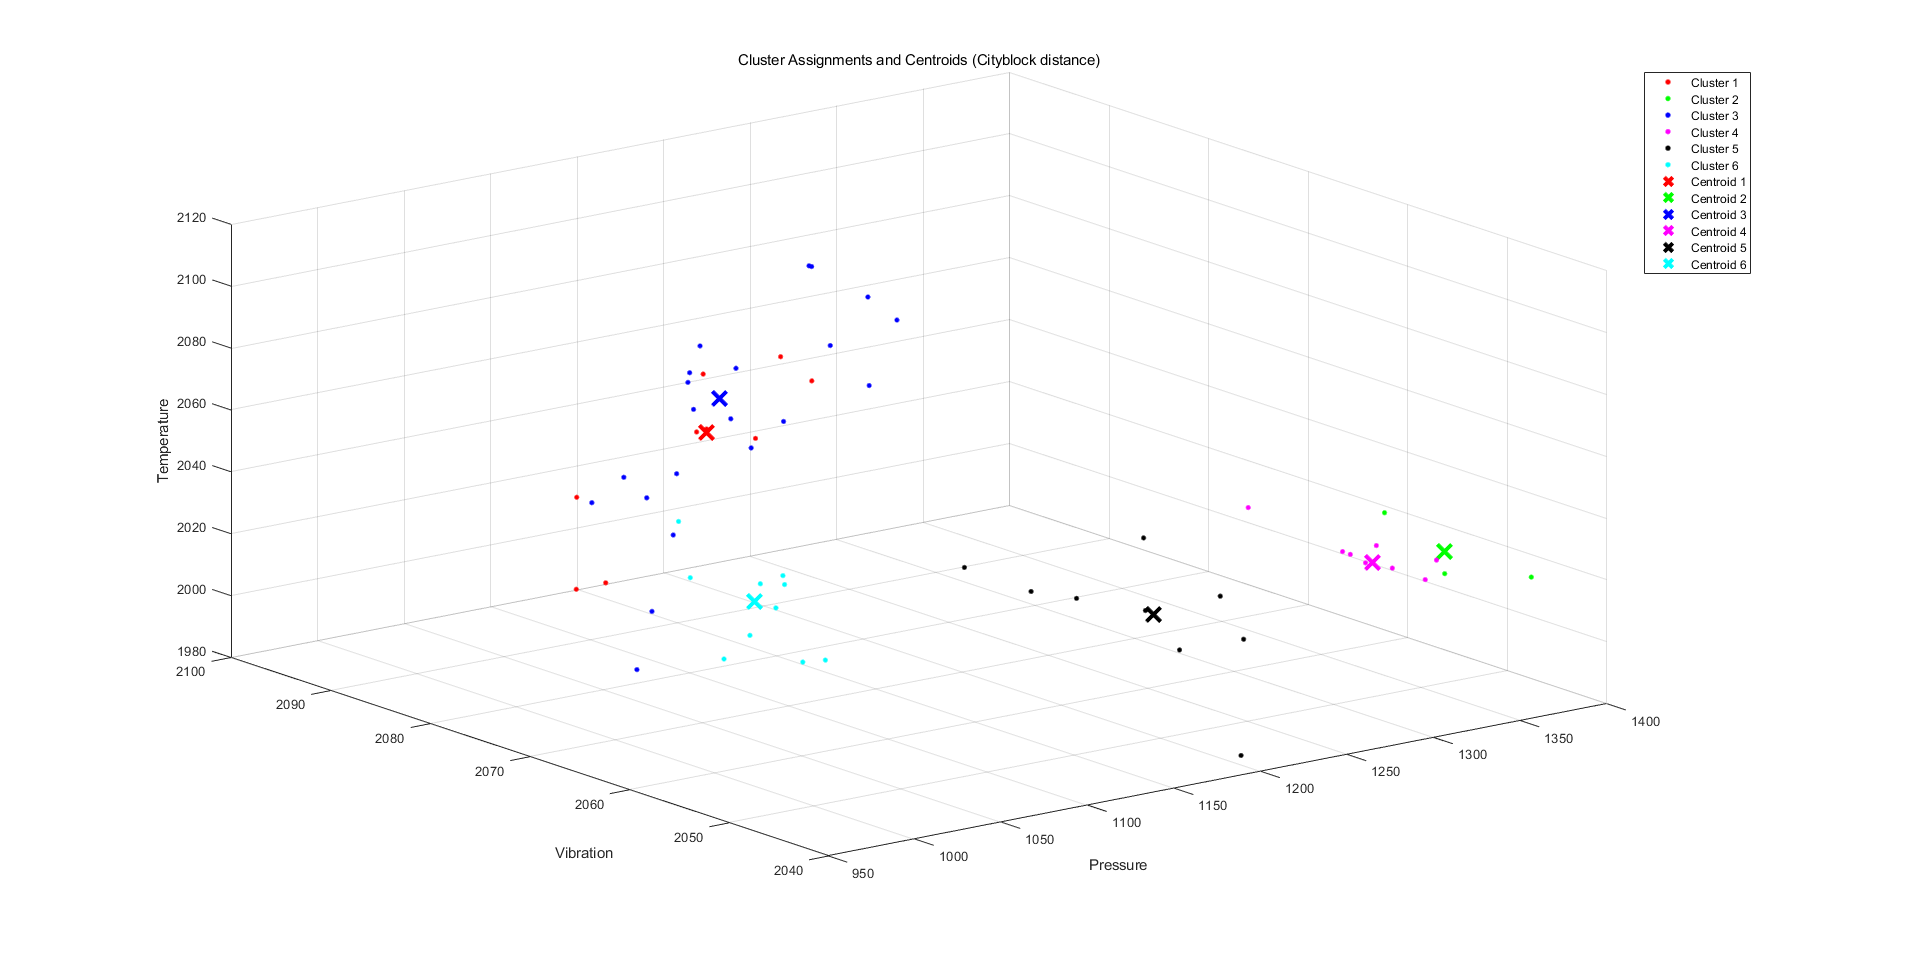
\includegraphics[width=0.47\textwidth]{sec4_part1c}
\end{center}
   \caption{K-means cluster algorithm with Cityblock distance}
\label{fig:31}
\end{figure}

\begin{figure}[h]
\begin{center}
   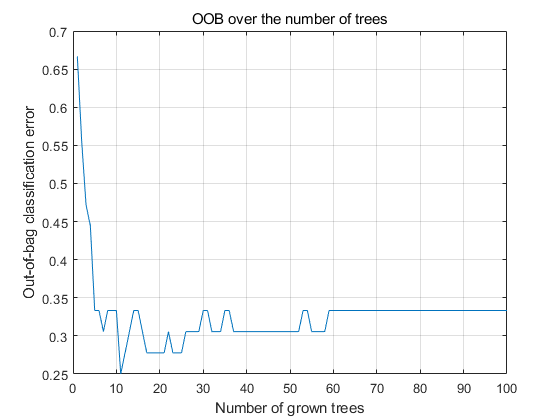
\includegraphics[width=0.47\textwidth]{sec4_part2a}
\end{center}
   \caption{OOB}
\label{fig:32}
\end{figure}

\begin{figure}[h]
\begin{center}
   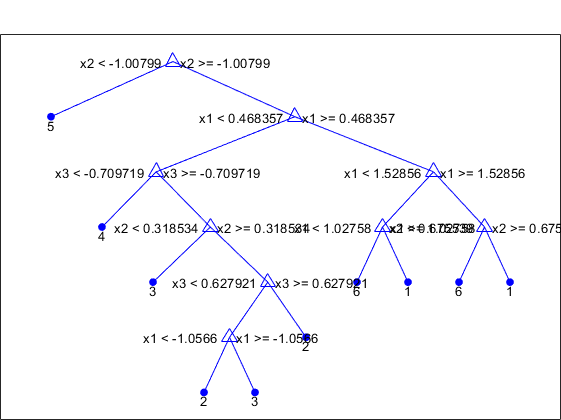
\includegraphics[width=0.47\textwidth]{sec4_part2b_1}
\end{center}
   \caption{The first decision tree among all 40 trees}
\label{fig:33}
\end{figure}

\begin{figure}[h]
\begin{center}
   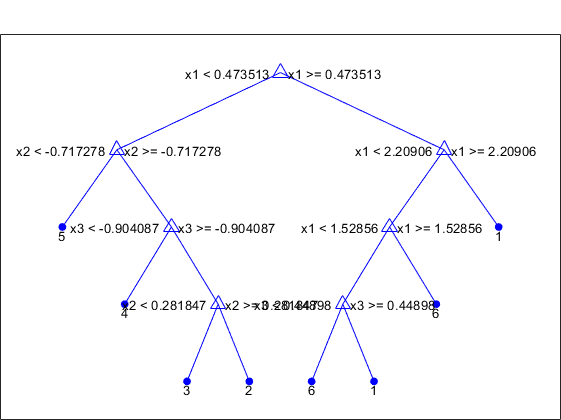
\includegraphics[width=0.47\textwidth]{sec4_part2b_2}
\end{center}
   \caption{The second decision tree among all 40 trees}
\label{fig:34}
\end{figure}

\begin{figure}[h]
\begin{center}
   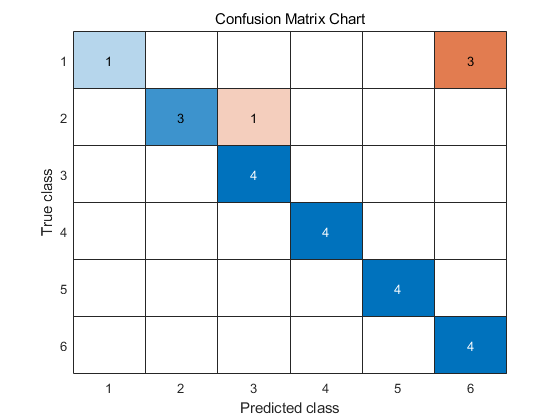
\includegraphics[width=0.47\textwidth]{sec4_part2c}
\end{center}
   \caption{Confusion matrix}
\label{fig:35}
\end{figure}


\end{document}
